% !TeX spellcheck = cs_CZ
%{\tikzset{external/prefix={tikz/FYZII/}}
% \tikzset{external/figure name/.add={ch05_}{}}
%---------------------------------------------------------------------------------------------------
% file fey1ch01_02_03.tex
%---------------------------------------------------------------------------------------------------
%====================Kapitola: Použití Gaussova zákona ============================================
\setchaptertoc
\chapter{Použití Gaussova zákona}\label{fyz:IIchapV}

V elektrostatice platí dva zákony: tok elektrického pole z objemu je přímo úměrný náboji v něm -
Gaussův zákon, a cirkulace elektrického pole je rovna nule, tj. \(\vec{E}\) je gradientem. Z těchto
dvou zákonů vyplývají v elektrostatice všechny předpovědi. Ale vyjádřit tyto zákony matematicky je
jedna věc a používat je snadno a s určitou dávkou důvtipu je věc druhá. V této kapitole probereme
řadu výpočtů, které je možné provést pomocí Gaussova zákona. Dokážeme některé věty a popíšeme
některé jevy, zejména ve vodičích, které je možno na základě tohoto zákona velmi snadno pochopit.
Samotný Gaussův zákon však nemůže poskytnout řešení žádné úlohy, neboť je třeba respektovat ještě
druhý zákon. Proto, když budeme používat Gaussův zákon k řešení konkrétních úloh, musíme k němu
ještě něco přidat: Budeme muset například udělat nějaký předpoklad o tom, jak vypadá pole, založený
například i na požadavcích symetrie. Anebo budeme muset explicitně zavést představu, že pole je
gradientem potenciálu \cite[s.~82]{Feynman02}.

\section{Rovnováha v elektrostatickém poli}\label{fyz:IIchapVsecI}
  Uvažujme nejdříve o tomto problému: Kdy může být bodový náboj ve stabilní mechanické rovnováze v
  elektrickém poli jiných nábojů? Jako příklad si představme tři záporné náboje umístěné ve
  vrcholech rovnostranného trojúhelníka ve vodorovné rovině. Zůstal by kladný náboj, který se
  nachází ve středu trojúhelníka, na tomto místě? (Bude jednodušší, když na okamžik zapomeneme na
  gravitaci, ačkoliv její zahrnutí výsledky stejně nezmění) Síla působící na kladný náboj je nulová,
  ale je to stabilní rovnováha? Vrátil by se náboj do rovnovážné polohy, kdyby se trochu posunul?
  Odpověď zní: ne.
  
  V \emph{žádném} elektrostatickém poli neexistují žádné body stabilní rovnováhy (s výjimkou poloh,
  ve kterých jsou už jiné náboje). Z Gaussova zákona je snadno vidět proč. Za prvé, má-li být náboj
  v rovnováze v nějakém konkrétním bodě \(P_0\), musí tam být pole nulové. Za druhé, má-li být
  rovnováha stabilní, požadujeme, aby při vysunutí náboje z \(P_0\) v jakémkoliv směru vznikla
  zpětná síla směřující opačně než posunutí. Elektrické pole tedy musí ve všech okolních bodech
  směřovat dovnitř - k bodu \(P_0\). Nejsou-li v \(P_0\) žádné náboje, bylo by to v rozporu s
  Gaussovým zákonem. Snadno se  můžeme přesvědčit.

  \begin{figure}[ht!] % \ref{fyz:fig186}
    \centering
    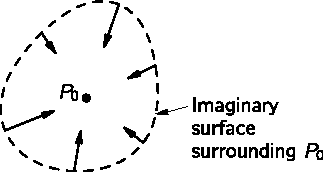
\includegraphics[width=0.6\linewidth]{fyz_fig186.pdf}
    \caption{Kdyby bod \(R\) představoval polohu stabilní rovnováhy kladného náboje, směřovalo  
      by elektrické pole všude v okolí k \(P_0\).}
    \label{fyz:fig186}
  \end{figure}
  Představme si malou myšlenou plošku, obklopující \(P_0\) (obr. \ref{fyz:fig186}). Směřuje-li všude
  v okolí elektrické pole do \(P_0\), jistě není plošný integrál normálové složky roven nule. V
  případě ukázaném na obrázku musí tok ploškou mít zápornou hodnotu. Podle Gaussova zákona tok
  elektrického pole z libovolné plochy je přímo úměrný celkovému náboji uvnitř. Není-li v \(P_0\)
  žádný náboj, je existence takového pole, jako jsme právě popsali, v rozporu s Gaussovým zákonem.
  Vyvážit kladný náboj v prázdném prostoru, tj. v bodě, v němž se nenachází žádný záporný náboj, se
  nepodaří. Kladný náboj může být v rovnováze jen tehdy, nachází-li še ve středu rozdělení záporného
  náboje. Samozřejmě, v takovém případě by rozdělení záporného náboje muselo být udržováno na místě
  jinými než elektrickými silami.
       
  Náš výsledek jsme získali pro bodový náboj. Platí tentýž závěr i pro složité uspořádání nábojů
  udržovaných pohromadě v pevných vzájemných polohách, řekněme tyčemi? Prozkoumáme tento problém pro
  dva stejné náboje upevněné na tyči. Může být v elektrostatickém poli takový útvar v rovnováze?
  Opět zní odpověď ne. Celková síla působící na tyč nemůže mít zpětný účinek pro posunutí v každém
  směru.
  
  Označme celkovou sílu působící na tyč v jakékoliv poloze \(\vec{F}\); \(\vec{F}\) je pak
  vektorovým polem. Budeme-li uvažovat jako předtím, dojdeme k závěru, že v poloze stabilní
  rovnováhy musí mít divergence \(\vec{F}\) zápornou hodnotu. Celková síla působící na tyč je rovna
  prvnímu náboji krát pole v jeho poloze, plus druhý náboj krát pole v jeho poloze: 
  \begin{equation}\label{fyz:eq_fey_elstat_gauss01}
   \vec{F}=q_1\vec{E_1} + q_2\vec{E_2}. 
  \end{equation}
  Pro divergenci \(F\) z toho vyplývá \[\ndiver{F}=q_1(\ndiver{E_1}) + q_2(\ndiver{E_2}).\] Je-li
  každý z těchto nábojů ve vakuu, jsou V \(q_1(\ndiver{E_1})\), stejně jako \(q_2(\ndiver{E_2})\)
  rovny nule a divergence \(\ndiver{F}\) je také rovna nule - není tedy záporná, jak by bylo žádoucí
  pro rovnováhu. Sami můžete rozšířit tuto úvahu a přesvědčit se, že vůbec žádný pevný útvar
  skládající se z jakéhokoliv počtu nábojů nemůže mít v elektrostatickém poli polohu stabilní
  rovnováhy ve volném prostoru.
  
  Nedokázali jsme však, že rovnováha je zakázána, existují-li úchyty nebo jiná mechanická omezení.
  Jako příklad nám poslouží dutá trubice, v níž se může náboj volně pohybovat dopředu a dozadu, ale
  ne do stran. V tomto případě je možno velmi snadno navrhnout elektrické pole, které na obou
  koncích směřuje dovnitř, připustí-li se, že v blízkosti středu trubice může směřovat ven do stran.
  Prostě na každý konec trubice umístíme kladné náboje, jak ukazuje obr. \ref{fyz:fig187}. Nyní může
  existovat rovnovážný bod i tehdy, když je divergence rovna nule. Náboj by, samozřejmě, nebyl ve
  stabilní rovnováze pro pohyb do stran, kdyby nepůsobily „neelektrické“ síly stěn trubice. 
  
  \begin{figure}[ht!] % \ref{fyz:fig187}
    \centering
    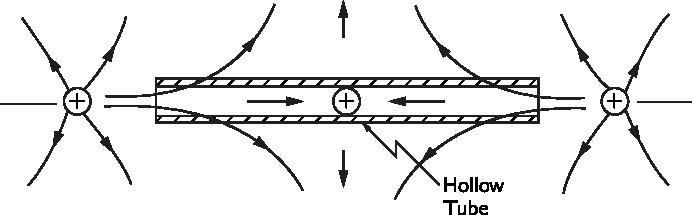
\includegraphics[width=0.7\linewidth]{fyz_fig187.pdf}
    \caption{Existují-li mechanické vazby, náboj může být v rovnováze.}
    \label{fyz:fig187}
  \end{figure}      
  
\section{Rovnováha s vodiči}\label{fyz:IIchapVsecII}
  V poli soustavy fixovaných nábojů neexistuje pro náš zkušební náboj žádná stabilní poloha. Jak je
  to v soustavě nabitých vodičů? Může soustava nabitých vodičů vytvořit takové pole, které bude mít
  bod stabilní rovnováhy pro bodový náboj? (Myslíme, samozřejmě, bod jinde než na povrchu vodiče.)
  Víte, že vodiče se vyznačují tím, že náboje v nich se mohou volně pohybovat. Je možné, že
  posune-li se trochu náš zkušební náboj, pohnou se ostatní náboje na vodičích tak, že na něj budou
  působit návratovou silou? Odpověď se stále stejná: Ne, ačkoliv z důkazu, který jsme podali výše,
  to není patrné. V tomto případě je důkaz těžší a my pouze naznačíme postup.
  
  \emph{Nejprve poznamenáme, že když se náboje na vodičích přerozdělují, může se to dít pouze tehdy,
  zmenšuje-li se tím jejich potenciální energie}. (Při pohybu ve vodiči se část jejich energie
  ztrácí na teplo). Už jsme ukázali, že jsou-li náboje vytvářející pole \emph{stacionární}, v
  blízkosti každého bodu \(P_0\), v němž je pole rovno nule, existuje takový směr, že posune-li se
  jím z \(P_0\), energie systému se zmenší (neboť síla směřuje od \(P_0\)). Jakékoliv přerozdělení
  nábojů na vodičích může pouze ještě víc zmenšit potenciální energii, takže (podle principu
  virtuální práce) jejich pohyb jen zvětší sílu ve zmíněném směru orientovanou od \(P_0\), ale
  neobrátí ji.
  
  Naše závěry neznamenají, že náboj není možné dostat do rovnováhy elektrickými silami. Je to možné,
  budou-li polohy nebo velikosti opěrných nábojů regulovány pomocí vhodných zařízení. Vy víte, že
  tyč postavená na hrot je v gravitačním poli nestabilní, ale to nedokazuje, že není možné ji
  vyvážit na konci prstu. Podobně je možné náboj udržovat v nějaké poloze elektrickými silami,
  jsou-li \emph{proměnné}. Ale ne pasivní, tj. \emph{statickou} soustavou sil.

\section{Stabilita atomů}\label{fyz:IIchapVsecIII}
  Nelze-li náboje trvale udržovat ve svých polohách, zajisté nebude adekvátní představovat si látku,
  jako kdyby se skládala ze statických bodových nábojů (elektronů a protonů), řídících se pouze
  zákony elektrostatiky. Taková elektrostatická konfigurace je nemožná, zhroutila by se.
  
  Svého času bylo navrženo, že kladný náboj atomu může být rozdělen homogenně v kouli a záporné
  náboje - elektrony mohou být v klidu uvnitř kladného náboje, jak je to znázorněno na obr.
  \ref{fyz:fig188}. To byl první model atomu, navržený Thomsonem. Na základě Geigerových a
  Marsdenových pokusů však dospěl Rutherford k závěru, že kladné náboje jsou velmi silně soustředěny
  v tom, co nazval \emph{jádrem}. Thomsonův statický model byl zavržen.
  \begin{figure}[ht!] % \ref{fyz:fig188}
    \centering
    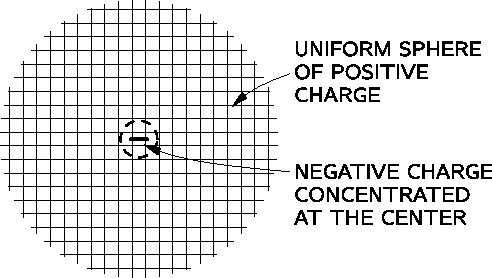
\includegraphics[width=0.6\linewidth]{fyz_fig188.pdf}
    \caption{Thomsonův model atomu}
    \label{fyz:fig188}
  \end{figure}
  
  Rutherford a Bohr pak navrhli, že půjde o dynamickou rovnováhu s elektrony obíhajícími na 
  orbitách, jako na obr. \ref{fyz:fig189}. Orbitální pohyb by zabraňoval 
  elektronům spadnout k jádru. Již známe nejméně jeden problém spojený s touto představou. Při 
  takovém pohybu by elektrony měly zrychlení (v důsledku jejich kruhového pohybu), a vyzařovaly 
  by proto energii.
  
  Tím by ztrácely kinetickou energii potřebnou na to, aby zůstaly na orbitě a spirálově by se 
  blížily k jádru. Opět nestabilita!
  \begin{figure}[ht!] % \ref{fyz:fig189}
    \centering
    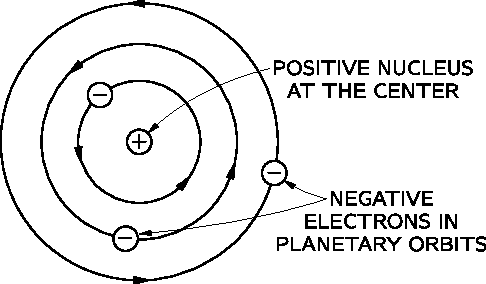
\includegraphics[width=0.6\linewidth]{fyz_fig189.pdf}
    \caption{Rutherfordův-Bohrův model atomu}
    \label{fyz:fig189}
  \end{figure}      
  
  Nyní se stabilita atomů vysvětluje pomocí kvantové mechaniky. Elektrostatické síly přitahují
  elektron těsně k jádru, jak je to jen možné, přičemž ten je však přinucen zůstat rozptýlen v
  prostoru do vzdálenosti vyplývající z principu neurčitosti. Byl-li by totiž omezen na příliš malý
  prostor, měl by velkou neurčitost v hybnosti. Ale to znamená, že by měl velkou střední energii,
  která by mu umožňovala vymanit se z elektrické přitažlivosti jádra. Konečným výsledkem je taková
  elektrická rovnováha, která se ani příliš neliší od Thomsonovy představy - pouze je to záporný
  náboj, který je rozptýlen (neboť hmotnost elektronu je mnohokrát menší než hmotnost protonu).

\section{Pole nabité přímky}\label{fyz:IIchapVsecIV}
  Gaussův zákon je možno použít na řešení mnoha úloh o elektrostatickém poli vyznačujících se
  speciální symetrií - obvykle kulovou, válcovou nebo rovinnou. Ve zbývající částí této kapitoly
  použijeme Gaussův zákon v několika takových úlohách. Snadnost, s jakou lze tyto úlohy takto řešit,
  může vést ke klamnému dojmu, že jde o velmi účinnou metodu umožňující postupovat tak i v mnoha
  dalších úlohách. Naneštěstí tomu tak není. Seznam úloh, které lze pomocí Gaussova zákona snadno
  řešit, bude brzy vyčerpán. V dalších kapitolách vypracujeme účinnější metody ke zkoumání
  elektrostatických polí.
  
  Jako náš první příklad budeme uvažovat soustavu s válcovou souměrností. Předpokládejme, že máme
  velmi dlouhou, homogenně nabitou tyč. Myslíme tím, že elektrické náboje jsou rovnoměrně rozděleny
  podél nekonečně dlouhé přímky, přičemž na \emph{jednotkovou délku} připadá náboj \(\tau\). Chceme
  vědět, jaké bude elektrické pole. Úlohu je jistě možno řešit integrováním příspěvků každé části
  přímky k poli. My to však dokážeme bez integrování, pomocí Gaussova zákona a důvtipu. Především
  snadno vytušíme, že elektrické pole bude směřovat radiálně od přímky. Jakákoli osová složka nábojů
  na jedné straně by se totiž anulovala stejně velkou osovou složkou pocházející od nábojů na straně
  druhé. Výsledkem může být pouze radiální pole. Také se zdá být odůvodněné, že pole by mělo mít
  tutéž velikost pro všechny body ve stejně velké vzdálenosti od přímky. Je to zřejmé. (Asi to není
  snadno dokazatelné, ale je to pravda, je-li prostor symetrický - a věříme, že je.)
  
  \luagraphic[0.9]{fyz_fig046.pdf}{Válcová gaussovská plocha s nabitou přímkou v ose}{fyz:fig046}

  Gaussův zákon můžeme použít následujícím způsobem. Mějme myšlenou válcovou plochu koaxiální s naší
  přímkou, jak to znázorňuje obr. \ref{fyz:fig046}. Podle Gaussova zákona je celkový tok pole z této
  plochy roven náboji uvnitř válce, dělenému \(\varepsilon_0\). Protože pole je na válcovou plochu
  kolmé, normálová složka pole je rovna velikosti pole. Označíme ji \(E\). Dále nechť poloměr válce
  je \(r\). Je výhodné brát jeho délku jako jednotkovou. Tok válcovou plochou je roven součinu \(E\)
  a jejího plošného obsahu, tj. \(2\pi r\). Tok oběma čelními stěnami je roven nule, protože
  elektrické pole je s nimi rovnoběžné. Celkový náboj uvnitř naší válcové plochy je přesně \(\tau\),
  neboť délka části přímky uzavřené uvnitř válce je rovna jedné jednotce. Z Gaussova zákona pak
  vyplývá, že
  \begin{equation}\label{fyz:eq_fey_elstat_gauss02}
    E\cdot2\pi r = \frac{\tau}{\varepsilon_0} \Rightarrow E = \frac{\tau}{2\pi\varepsilon_0 r}
  \end{equation}
  Elektrické pole nabité přímky je nepřímo úměrné \emph{první} mocnině vzdálenosti od přímky.
  
    %---------------------------------------------------------------
     % !TeX spellcheck = cs_CZ
\begin{mdframed}[style=mdexam]
  \begin{example}\label{fyz:fey_exam001}
    \href{http://librarian/stable.php?id=380}{Soustředné válce}: Velmi tenký nevodivý plášť válce o
    poloměru \(b\) a délce \(L\) obklopuje dlouhý, plný nevodivý válec o poloměru \(a\) a délce
    \(L\), kde \(b < a\). V celém objemu vnitřního válce je spojitě vyplněn nábojem o celkové
    velikosti \(+Q\). Na povrchu vnějším plášti válce je spojitě rozprostřen náboj stejné velikosti,
    opačného znaménka \(−Q\). Oblast \(a < r < b\) je prázdná. S využitím Gaussova zákona určete
    intenzitu elektrického pole v celém prostoru.
      
    {\centering
    \captionsetup{type=figure}
    \luafigure[0.5]{fyz_fig0212.pdf}
    \captionof{figure}{K příkladu \ref{fyz:fey_exam001}
    \label{fyz:fig0212}}
    \par}
    
    \begin{enumerate}[noitemsep]
      \item \emph{Jaká je symetrie úlohy?} Cylindrická
      \item \emph{Jaký je směr intenzity elektrického pole?} Vektor intenzity elektrické pole míří v
            radiálním směru cylindrické vztažné soustavy, jeho velikost je konstantní na
            cylindrických plochách s konstantním poloměrem. 
      \item \emph{Kolik různých oblastí v prostoru budeme vyšetřovat?} Budeme vyšetřovat tři
             oblasti, uvnitř \(a\), mezi \(a\) a \(b\), vně \(b\).
      \item \emph{Pro každou oblast v prostoru zvolte Gaussovu plochu, jakou proměnnou zvolíte pro
            parametrizaci těchto ploch? Jaké jsou obory hodnot této proměnné?} V každé oblasti
            budeme používat válcové plochy o poloměru \(r\) a výšce \(h\), které jsou souosé se
            skutečnými válci. Plochu budeme popisovat poloměrem \(r\), jehož obor hodnot je interval
            \(\left\langle 0,\infty\right)\).
      \item \emph{Pro oblast \(r < a\) spočítejte tok Gaussovou plochou, kterou jste si vybrali. Ve
            vyjádření by jste měli mít i neznámou intenzitu elektrického pole.} Obě podstavy
            Gaussova válce nebudou přispívat k celkovému toku plochou (ze symetrie je pole
            rovnoběžné s touto plochou). Tok pláštěm válce tak je
            \begin{equation*}
              \Phi_E = \oiint\vec{E}\dd{S} = 2\pi r h E.
            \end{equation*}
            \item \emph{Pro oblast r < a spočítejte náboj uzavřený ve zvolené Gaussově ploše.}
            Ve vnitřním válci je náboj homogenně rozložen. Náboj uzavřený v Gaussově ploše můžeme
            vyjádřit dvěma způsoby: (1) jako objemový podíl uzavřený v ploše nebo (2) využitím
            objemové nábojové hustoty \(\varrho\). Výpočet je proveden oběma způsoby:
            \begin{enumerate}[noitemsep]
              \item \(Q_{in} = \dfrac{V_{in}}{V_{total}}Q = \dfrac{r^2h}{a^2L}Q\)
              \item \(\varrho = \dfrac{Q}{L\pi a^2} 
                    \Rightarrow Q_{in} = \varrho\pi r^2h = \dfrac{r^2h}{a^2L}Q\)
            \end{enumerate}
      \item \emph{Pro oblast \(r < a\) dejte podle Gaussova zákona do rovnosti vztahy z 5. a 6.
            bodu, vyjádřete velikost intenzity elektrického pole.}
            \begin{equation*}
              2\pi r h E = \frac{1}{\varepsilon_0}\dfrac{r^2h}{a^2L}Q 
              \Rightarrow E = \frac{Qr}{2\pi\varepsilon_0a^2L}
            \end{equation*}
            \emph{Zopakujte stejnou proceduru pro oblast \(a < r < b\), vyjádřete intenzitu
            elektrického pole jako funkci \(r\).} Náboj, který je uzavřen v ploše je konstantní, se
            vzrůstajícím poloměrem r se však mění celková plocha válce.
            \begin{equation*}
              2\pi\,r\,h\,E = \frac{1}{\varepsilon_0}\dfrac{h}{L}Q 
              \Rightarrow E = \frac{Q}{2\pi\varepsilon_0rL}
            \end{equation*}
      \item Zakreslete \emph{intenzitu elektrického pole} jako graf funkce v závislosti na
            parametru, který popisoval Gaussovou plochu. Graf nakreslete pro celý prostor. 
            
            {\centering
              \captionsetup{type=figure}
              \luafigure[0.9]{fyz_fig0213.pdf}
              \captionof{figure}{K příkladu \ref{fyz:fey_exam001}
              \label{fyz:fig0213}}
              \par}
      \item Jaký je \emph{rozdíl potenciálů} mezi body \(r = a\) a \(r = 0\)? Tedy, kolik je
            \(\Delta V = V(a) − V(0)\)? 
            \begin{align*}
              \Delta V  &= V(a) − V(0) = -\int_0^a\vec{E}(r)\dd\vec{r}   \\
                        &= -\int_{0}^{a}E(r)\vec{r}\cdot\vec{r}\dd{r}    \\
                        &= -\int_{0}^{a}\frac{Qr}{2\pi\varepsilon_0a^2L} 
                         = -\frac{Q}{2\pi\varepsilon_0L}
            \end{align*}
      \item Jaký je rozdíl potenciálů mezi body \(r = b\) a \(r = a\)?
            \begin{align*}
              \Delta V  &= V(b) − V(a) = -\int_a^b\vec{E}(r)\dd\vec{r} \\   
                        &= -\int_a^b E(r)\vec{r}\cdot\vec{r}\dd{r}     \\
                        &= -\int_a^b \frac{Q}{2\pi\varepsilon_0rL} 
                         = -\frac{Q}{2\pi\varepsilon_0L}\ln\frac{b}{a}
            \end{align*}
            Opět je rozdíl potenciálů záporný, neboť potenciál v místě \(r = a\) je vyšší než v
            místě \(r = b\).
    \end{enumerate}
  \end{example}
\end{mdframed}
    %---------------------------------------------------------------

\section{Nabitá rovina, dvě roviny}\label{fyz:IIchapVsecV}
  V dalším příkladě budeme počítat pole homogenně nabité roviny. Předpokládejme, že rovina se
  rozprostírá do nekonečna a na její plošnou jednotku připadá náboj \(\sigma\). Teď provedeme další
  odhad. Důvody souměrnosti nás totiž vedou k přesvědčení, že směr pole je všude kolmý na rovinu a
  že \emph{neexistuje-li pole jiných nábojů}, musí být pole na obou stranách roviny stejné (co do
  velikostí). Tentokrát zvolme jako naši gaussovskou plochu pravoúhlou krabičku, která protíná
  uvažovanou rovinu (obr. \ref{fyz:fig191}). Stěny krabičky rovnoběžné s rovinou budou mít stejný
  plošný obsah \(S\). Pole je na tyto dvě stěny kolmé a se zbývajícími čtyřmi stěnami je rovnoběžné.
  Celkový tok je roven \(E-\text{krát}\) plošnému obsahu první stěny plus \(E-\text{krát}\) plošný
  obsah protilehlé stěny, přičemž zbývající čtyři stěny nepřispívají ničím. Celkový náboj uvnitř
  krabičky je \(\sigma\cdot S\). Když jej uvedeme do vztahu s tokem stěnami krabice, dostaneme
  rovnost
  \begin{equation}\label{fyz:eq_fey_elstat_gauss03}
    E\cdot S + E\cdot S = \frac{\sigma\cdot S}{\varepsilon_0} \Rightarrow 
    E = \frac{\sigma}{2\varepsilon_0}.
  \end{equation}
  
  \begin{figure}[ht!] % \ref{fyz:fig191}
    \centering
    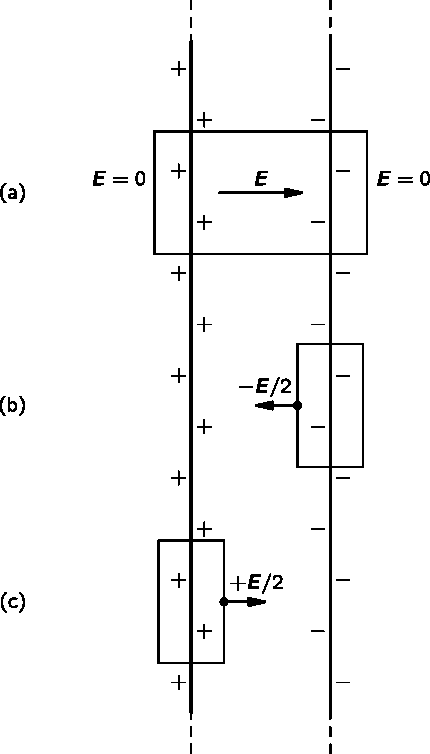
\includegraphics[width=0.6\linewidth]{fyz_fig191.pdf}
    \caption{Elektrické pole v blízkosti homogenně nabité roviny je možno najít použitím   
             Gaussova zákona na myšlenou krabici.}
    \label{fyz:fig191}
  \end{figure}
  
  Tentýž výsledek jsme dostali už dříve integrováním po celé ploše. Gaussův zákon nám dává odpověď v
  tomto příkladě o mnoho rychleji (ačkoli nemá takovou obecnou použitelnost jako dřívější metoda).

  \begin{figure}[ht!]  %\ref{fyz:fig192}
    \centering
    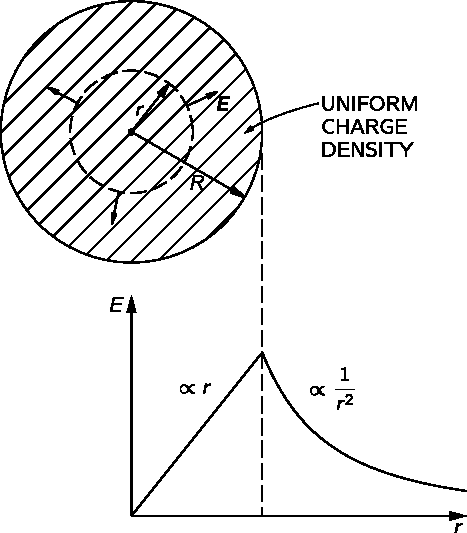
\includegraphics[width=0.6\linewidth]{fyz_fig192.pdf}
    \caption{Pole mezi dvěma nabitými rovinami je rovno \(\dfrac{\sigma}{\varepsilon_0}\)}
    \label{fyz:fig192}
  \end{figure}
  Zdůrazňujeme, že tento výsledek se vztahuje pouze na pole vytvořené náboji rozmístěnými v rovině.
  Nacházejí-li se někde v blízkostí ještě další náboje, bude celkové pole v okolí roviny rovno
  součtu pole (\ref{fyz:eq_fey_elstat_gauss03}) a pole pocházejícího od těchto nábojů.
   
  Úloha se dvěma rovnoběžnými rovinami se stejnými plošnými hustotami nábojů, které mají opačná
  znaménka \(+\sigma\) a \(-\sigma\), je také jednoduchá, předpokládáme-li opět, že vnější svět je
  zcela souměrný. Superpozicí obou řešení pro jednotlivé roviny nebo sestrojením gaussovské krabice,
  která by proťala obě roviny, je možno jednoduše ozřejmit, že na vnější straně rovin je pole rovno
  nule (obr. \ref{fyz:fig192}a). Kdybychom uvažovali krabici, která protíná jen jednu z rovin částí
  b, c obrázku), mohli bychom se přesvědčit, že pole mezi deskami musí být dvakrát větší než v
  případě jedni desky. Podle Gaussova zákona by pak platilo, že
  \begin{equation}\label{fyz:eq_fey_elstat_gauss04}
    E_1 + E_2 = \frac{\sigma}{\varepsilon_0}
  \end{equation}
  kde \(E_1\) a \(E_1\) jsou pole na každé straně roviny směřující od ní.

  Máme tedy výsledek
  \begin{align}
    E (\text{mezi deskami}) &= \frac{\sigma}{\varepsilon_0} \\
    E (\text{venku})        &= 0  
  \end{align}
  
\section{Nabitá koule, kulová slupka}\label{fyz:IIchapVsecVI}
  V kapitole \ref{fyz:IIchapIVsecVII} jsme již použili Gaussův zákon k nalezení pole v okolí
  homogenně nabité kulové slupky. Touž metodou je možné získat pole i ve vnitřních bodech koule.
  Tento výpočet je například možné použít k získání dobrého přiblížení pole uvnitř atomového jádra.
  Přesto, že se protony v jádře navzájem odpuzují, jsou působením velkých jaderných sil v objemu
  jádra rozptýlené zhruba homogenně.

  \begin{figure}[ht!]  %\ref{fyz:fig047}
    \centering
    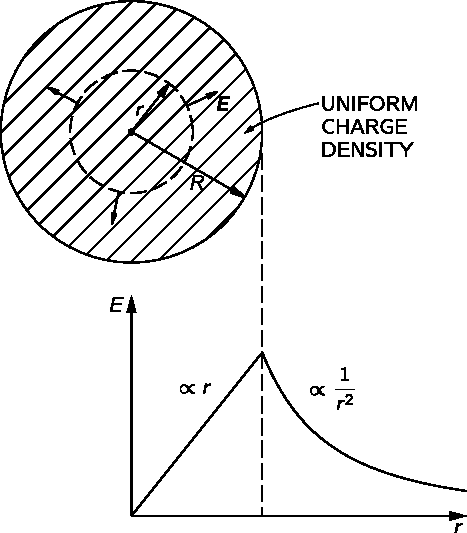
\includegraphics[width=0.7\linewidth]{fyz_fig047.pdf}
    \caption{Gaussův zákon je možno použít k nalezení pole uvnitř homogenně nabité koule.}
    \label{fyz:fig047}
  \end{figure}
  Mějme kouli s poloměrem \(R\), homogenně vyplněnou nábojem. Nechť \(\varrho\) je náboj v jednotce
  objemu. Na základě souměrnosti opět předpokládejme, že pole bude radiální, a ve všech bodech
  stejně vzdálených od středu koule bude mít tutéž velikost. Abychom našli pole ve vzdálenosti \(r\)
  od středu, vložíme dovnitř koule soustřednou gaussovskou plochu s poloměrem \(r\) \((r< R)\), jak
  to ukazuje obr. \ref{fyz:fig047}. Tok z této plochy je 
  \[4\pi r^2E.\]

  Náboj uvnitř plochy je roven jí uzavřenému objemu vynásobenému hustotou \(\varrho\):
  \begin{equation}\label{fyz:eq_fey_elstat_gauss05} 
    Q_{\text{uvnitř}} 
            = \limitint_{\mathclap{\substack{\text{objem}\\
                                             \text{uvnitř }S}}} \varrho\dd{V} 
            = \frac{4}{3}\pi r^3\varrho.           
  \end{equation}
  Z Gaussova zákona pak pro velikost pole vyplývá vztah:
  \begin{align}      
   \limitint_S E_n\dd{S}
      &= \frac{Q_{\text{uvnitř}}}{\varepsilon_0} 
            \quad\Rightarrow\quad 4\pi r^2E 
            = \frac{4\pi r^3\varrho}{3\,\varepsilon_0}  \label{fyz:eq_fey_elstat_gauss06} \\ 
   \shortintertext{tedy:}
   E  &= \frac{\varrho r}{3\,\varepsilon_0} \quad (r<R).
  \end{align}
  
  Můžete se přesvědčit, že tento vztah dává správný výsledek i pro \(r=R\). Elektrické pole je přímo
  úměrné vzdálenosti od středu koule, má směr poloměru a je orientované směrem ven od středu. Úvahy,
  které jsme právě dělali pro homogenně nabitou kouli, je možno aplikovat i na tenkou nabitou
  kulovou slupku. Uděláme-li předpoklad, že pole je všude radiální a kulově symetrické, z Gaussova
  zákona okamžitě vyplyne, Že pole na vnější straně slupky je podobné poli bodového náboje, zatímco
  všude uvnitř je rovno nule. (Gaussovská plocha uvnitř slupky nebude obklopovat žádný náboj.)
  
\section{Je pole bodového náboje přesně přímo úměrné veličině 
             \texorpdfstring{\fontsize{8pt}{9pt}\selectfont\(\dfrac{1}{r^2}\)}{1/r^2}?}\label{fyz:IIchapVsecVII}
              
  Podíváme-li se trochu podrobněji, jak se pole uvnitř kulové slupky stává nulovým, lépe si
  ozřejmíme, proč platnost Gaussova zákona vyplývá právě jen z přesné závislosti Coulombovy síly na
  druhé mocnině vzdálenosti. Uvažujme nějaký bod \(P\) uvnitř homogenně nabité kulové plochy.
  Představme si úzký kužel, který má vrchol v \(P\) a sahá po kulovou plochu, na které vytíná malou
  plošku s plošným obsahem \(\Delta S_1\) (obr. \ref{fyz:fig193}). S ním přesně souměrný kužel
  vycházející z \(P\) na opačnou stranu by na kulové ploše vyřízl plošku s obsahem \(\Delta S_2\).
  Jsou-li vzdálenosti od \(P\) k těmto dvěma ploškám \(r_1\) a \(r_2\), jsou jejich plošné obsahy v
  poměru \[\frac{\Delta S_2}{\Delta S_1} = \frac{r_2^2}{r_1^2}\] (To můžete dokázat pomocí geometrie
  pro jakýkoliv bod \(P\) uvnitř koule).

  \begin{figure}[ht!] % \ref{fyz:fig193}
    \centering
    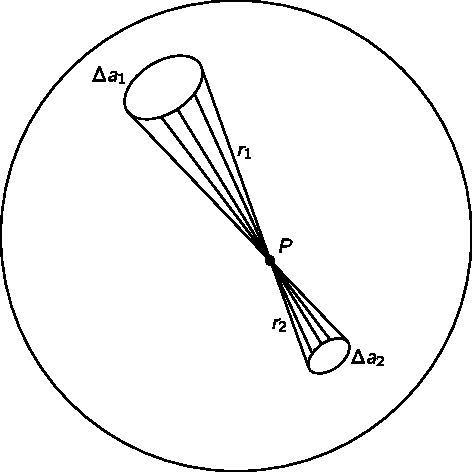
\includegraphics[width=0.6\linewidth]{fyz_fig193.pdf}
    \caption{V každém bodě \(P\) uvnitř nabité kulové plochy je pole nulové.}
    \label{fyz:fig193}
  \end{figure}
  Je-li povrch koule homogenně nabitý, je náboj \(\Delta q\) na každé vyříznuté plošce přímo úměrný
  její velikosti, tedy \[\frac{\Delta q_2}{\Delta q_1} = \frac{\Delta S_2}{\Delta S_1}.\]
  
  Podle Coulombova zákona velikosti polí vytvořených těmito dvěma ploškami v bodě \(P\) jsou v
  poměru \[\frac{E_2}{E_1} = \frac{q_2/r_2^2}{q_1/r_1^2} = 1.\]
  
  Obě pole se přesně ruší. Protože takové dvojice plošek je možné vytvořit že všech Částí kulové
  plochy, je výsledné pole v \(P\) rovno nule. Můžeme se však přesvědčit, že by to tak nebylo, kdyby
  mocnina \(r\) v Coulombově zákoně nebyla rovna přesně dvěma.
  
  Platnost Gaussova zákona je podmíněna nepřímou úměrností druhé mocnině vzdálenosti v Coulombově
  zákoně. Neob\-sahoval-li by zákon ve jmenovateli přesně druhou mocninu, neplatilo by, že pole
  uvnitř homogenně nabité kulové plochy je přesně rovno nule. Kdyby se například pole měnilo
  rychleji, řekněme nepřímo úměrně třetí mocnině \(r\), ta část plochy, která je blíž k uvažovanému
  vnitřnímu bodu, by v něm vytvářela větší pole než ta část, která je od něho dál. Výsledkem by bylo
  radiální pole směřující v případě kladného náboje do středu koule. Tyto závěry nám napovídají
  elegantní způsob jak zjistit, zda zákon o nepřímé úměrnosti druhé mocnině platí přesně.
  Potřebujeme pouze zjistit, zda je pole uvnitř homogenně nabité kulové plochy přesně rovno nebo
  nerovno nule.
  
  Je štěstí, že taková metoda existuje. Obvykle je těžké změřit fyzikální veličinu s vysokou 
  přesností. Dosáhnout výsledku s chybou jedno procento by asi příliš těžké nebylo, ale jak 
  měřit, řekněme, Coulombův zákon s přesností na jednu miliardtinu? Téměř jistě není možné ani 
  pomocí nejlepších existujících přístrojů měřit s takovou přesností sílu mezi dvěma nabitými 
  tělesy. Ale budeme-li určovat pouze to, zda jsou elektrická pole uvnitř nabité koule menší 
  než nějaká hodnota, můžeme tím udělat velmi přesné měření platnosti Gaussova zákona a tedy 
  závislosti na druhé mocnině vzdálenosti ve jmenovateli Coulombova zákona. Efektivně se tím 
  provede porovnání zákona síly s ideální nepřímou úměrností druhé mocnině vzdálenosti. Na 
  takových porovnáváních stejných nebo přibližně stejných věcí se obvykle zakládají ta 
  nejpřesnější fyzikální měření.
  
  Jak pozorovat pole uvnitř nabité koule? Jeden způsob je zkusit nabít nějaké těleso tak, že se 
  jím dotkneme nitra kulového vodiče. Víte, že dotkneme-li se nabitého tělesa kovovou kuličkou 
  a pak sejí dotkneme elektrometru, ten se nabije a jeho ručička se vychýlí z nulové polohy 
  (obr. \ref{fyz:fig194a}). Kulička nabírá náboj, neboť elektrické síly v okolí 
  nabité koule ženou náboje na kuličku (nebo z ní). Provedeme-li pokus tak, že se kuličkou 
  dotýkáte nitra nabité koule, zjistíme, že na elektrometr se nepřenáší žádný náboj. Pomocí 
  takového pokusu můžete také snadno dokázat, že pole uvnitř dosahuje nanejvýš několika procent 
  vnějšího pole a že Gaussův zákon je alespoň přibližné správný \cite[s.~91]{Feynman02}.
  \begin{figure}[hb!]
    \centering
    \subcaptionbox{\label{fyz:fig194a}}{\luafigure[0.45]{fyz_fig194a.pdf}}
    \subcaptionbox{\label{fyz:fig194b}}{\luafigure[0.45]{fyz_fig194b.pdf}}                      
    \caption{Uvnitř uzavřené kulové plochy je elektrické pole všude rovno nule.}
    \label{fyz:fig194}
  \end{figure}
    
  Zdá se, že prvním, kdo zjistil, že pole uvnitř vodivé slupky je rovno nule, byl Benjamin 
  Franklin. Připadalo mu to divné. Když svůj poznatek oznámil Priestleyovi, ten navrhl, že 
  mohlo souviset se zákonem nepřímé úměrnosti druhé mocnině vzdálenosti, neboť bylo známo, že 
  kulová hmotná slupka uvnitř nevytváří žádné gravitační pole. Ale Coulomb naměřil nepřímou 
  úměrnost druhé mocnině vzdálenosti až o 18 let později a Gaussův zákon byl objeven ještě 
  později.
  
  Gaussův zákon byl pečlivě prověřován. Za tímto účelem se elektrometr umístil uvnitř velké 
  koule a sledovalo se, zda se neobjeví nějaké výchylky, když se koule nabije na vysoké napětí. 
  Vždy bylo dosaženo záporného výsledku. Z geometrie aparatury a citlivosti elektrometru je 
  možné vypočítat, jaké nejmenší pole by se projevilo. Z této hodnoty lze stanovit horní 
  ohraničení odchylky mocnitele od dvou. Napíšeme-li, že elektrostatická síla je úměrná 
  \(r^{2+\varepsilon}\), můžeme určit horní hranici pro \(\varepsilon\). Touto metodou Maxwell 
  určil, že \(\varepsilon\) je méně než \(\num{1/10 000}\). V roce 1936 Plimpton a Laughton 
  experiment zopakovali a zdokonalili. Zjistili, že mocnitel se liší od dvou o méně než jednu 
  miliardtinu.
  
  To nás přivádí k zajímavé otázce: Do jaké míry víme, jak přesně platí Coulombův zákon v 
  různých situacích? Právě popsané pokusy měří závislost pole na vzdálenosti řekněme několika 
  desítek centimetrů. Ale co třeba vzdálenosti uvnitř atomu, např. vodíkového atomu, v němž, 
  jak předpokládáme, je elektron přitahován k jádru podle téhož zákona nepřímé úměrnosti druhé 
  mocnině vzdálenosti? Je pravda, že k popisu mechanické stránky chování elektronu musí být 
  použita kvantová mechanika, ale přitom jde o obyčejnou elektrostatickou sílu. Při formulování 
  úlohy o atomu vodíku je potřeba znát potenciální energii elektronu jako funkci vzdálenosti od 
  jádra. Coulombův zákon dává potenciál, který se mění nepřímo úměrně první mocnině 
  vzdálenosti. S jakou přesností je znám mocnitel pro takové malé vzdálenosti? Z velmi 
  pečlivých měření relativních poloh energetických hladin vodíku, které provedli Lamb a 
  Retherford r. 1947, víme, že v rozměrech atomu, tj. ve vzdálenostech řádově desetin nanometru 
  (\SI{10e-10}{\meter}), Souhlasí mocnitel opět s přesností jedné miliardtiny.
  
  Přesnost Lambova-Retherfordova měření znovu umožnila fyzikální „náhoda“. Ze stavů atomu 
  vodíku by dva měly mít téměř stejné energie, ale jen tehdy, mění-li se potenciál přesně jako 
  \(1/r\). Tento velmi malý rozdíl jejich energií se měřil zjišťováním úhlové frekvence 
  \(\omega\) fotonů emitovaných nebo absorbovaných při přechodech mezi těmito dvěma stavy na 
  základě vztahu pro rozdíl energie \(\Delta E = \si{\planckbar}\omega\)). Výpočty ukázaly, že 
  \(\delta E\) by se zřetelně odlišovalo od naměřené hodnoty, kdyby se mocnitel v zákoně síly 
  \(1/r^2\) lišil od dvou už o víc než jednu miliardtinu.
  
  Je tentýž mocnitel správný i pro kratší vzdálenosti? Z měření v jaderné fyzice se zjistilo, 
  že v typických jaderných vzdálenostech, zhruba \SI{10e-15}{\meter}, se uplatňují 
  elektrostatické síly a také se mění jako převrácená hodnota druhé mocniny vzdálenosti. Na 
  některé z důkazů, které o tom svědčí, se podíváme později. Víme tedy, že Coulombův zákon 
  ještě platí, alespoň v takové míře, i pro vzdálenosti řádu \SI{10e-10}{\meter}.
  
  A co při \SI{10e-16}{\meter}? Tento dosah je možné zkoumat ostřelováním protonů elektrony s 
  velmi vysokou energií a pozorováním jejich rozptylu. Jak se zdá, získané údaje naznačují, že 
  při těchto vzdálenostech zákon selže. Elektrická síla se ukazuje být ve vzdálenostech menších 
  než \SI{10e-16}{\meter} asi 10-krát slabší. Jsou dvě možná vysvětlení. Jedno je, že v 
  takových malých vzdálenostech Coulombův zákon neplatí. Druhé je, že naše „tělesa“, tj. 
  protony a elektrony, nepředstavují bodové náboje. Možná že elektron nebo proton nebo oba jsou 
  nějak rozmazány. Většina fyziků se domnívá, že rozmazán je náboj protonu. Víme, že protony 
  silně interagují s mezony. To předpokládá, že proton čas od času existuje jako neutron s 
  mezonem \(\pi^+\) kolem sebe. V průměru bude takováto konfigurace působit jako malá kulička 
  kladného náboje. Víme, že pole nabité koule se při postupu do jejího středu nemění stále jako 
  \(1/r^2\). Je docela pravděpodobné, že náboj protonu je rozmazaný, ale i teorie 
  \(\pi\text{-mezonů}\) je ještě dost nedokonalá, takže možná i Coulombův zákon selže na velmi 
  malých vzdálenostech\footnote{Experimenty, které Feynman popisuje, postupně vedly k dnešní 
  představě, podle níž protony, neutrony i mezony skutečně nejsou bodové částice, ale mají 
  vnitřní strukturu tvořenou kvarky. Kvarky přitom nemohou existovat samostatně.}.
  
  Ještě jedna věc: zákon nepřímé úměrnosti druhé mocnině vzdáleností platí pro vzdálenosti řádu 
  \SI{1}{\meter}, ale i pro \newline\SI{10e-10}{\meter}; zůstává však činitel 
  \(\dfrac{1}{4\pi\varepsilon_0}\) stále stejným? Odpověď je ano, alespoň s relativní přesností 
  15 milióntin.
  
  Nyní se vraťme k důležitému problému, který jsme přešli mlčením, když jsme hovořili o 
  experimentálním potvrzení Gaussova zákona. Možná, že jste se podivili, jak mohl být výsledek 
  experimentu Maxwella nebo Plimptona a Lauglitona tak přesný, když přitom kulový vodič, který 
  použili, nebyl dokonalou koulí. Vždyť dosáhnout přesnosti na jednu miliardtinu je už opravdu 
  něco a právem byste se mohli ptát, zda dokázali udělat tak přesnou kouli. Každá reálná koule 
  má určitě malé nepravidelností. Existují-li nepravidelnosti, nebudou uvnitř vytvářet pole? 
  Nyní chceme ukázat, že není třeba mít dokonalou kouli. Opravdu lze dokázat, že uvnitř 
  uzavřené vodivé plochy jakéhokoliv tvaru není žádné pole. Jinými slovy, výsledek zmíněných 
  experimentů závisel na \(1/r^2\), ale vůbec ne na tom, zda je plocha kulová (až na to, že pro 
  kouli je snazší vypočítat, jaká by byla pole, kdyby Coulombův zákon neplatil), a tak se nyní 
  vracíme znovu k našemu problému. Abychom to ukázali, je nevyhnutelné poznat některé 
  vlastností elektrických vodičů.
  
\section{Pole vodiče}\label{fyz:IIchapVsecVIII}
  Elektrickým vodičem je pevné těleso, které obsahuje mnoho „volných“ elektronů. Elektrony se 
  mohou v tělese volně pohybovat, ale nemohou projít jeho povrchem. V kovu je tolik volných 
  elektronů, že jakékoliv elektrické pole jich uvede do pohybu velké množství. Takto vzniklý 
  proud elektronů se pak musí buď udržovat vnějšími zdroji energie, nebo se pohyb elektronů 
  zastaví, jakmile elektrony vybijí zdroje, které vytvořily původní pole. V elektrostatice 
  nepracujeme se stálými zdroji proudu (jimi se budeme zabývat později, až budeme hovořit o 
  magnetostatice), takže elektrony se pohybují jen dokud se neuspořádají tak, aby všude uvnitř 
  vodiče vytvořily nulové elektrické pole. (Obvykle se to stane v malém zlomku sekundy). Kdyby 
  totiž ještě nějaké pole zůstalo, uvedlo by do pohybu další elektrony; jediným možným řešením 
  v elektrostatice je, že je pole uvnitř vodiče je všude nulové.
  
  Nyní si všimněme vnitřku nabitého vodivého tělesa. („Vnitřkem“ rozumíme prostor v objemu 
  kovu.) Protože kov je vodič, vnitřní pole, a tedy gradient potenciálu \(\varphi\) musí být 
  roven nule. Každý vodič tak představuje ekvipotenciální oblast a jeho povrch je 
  ekvipotenciální plochou. Protože všude ve vodivé látce je elektrické pole rovno nule, je nule 
  rovna i divergence \(\vec{E}\) a podle Gaussova zákona musí být rovna nule i hustota náboje 
  uvnitř vodiče.

  \begin{figure}[ht!]  % \ref{fyz:fig195}
    \centering
    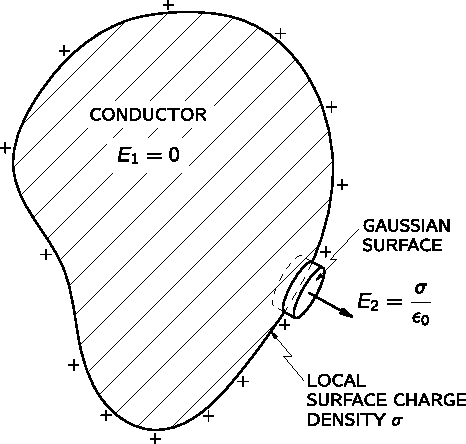
\includegraphics[width=0.7\linewidth]{fyz_fig195.pdf}
    \caption{Elektrické pole těsně při povrchu vodiče je přímo úměrné lokální plošné hustotě  
             náboje na povrchu.}
    \label{fyz:fig195}
  \end{figure} 
  Nemohou-li být ve vodiči žádné náboje, jak je možné jej nabít? Co máme na mysli, když říkáme, 
  že je vodič „nabit“? Kde tedy náboje jsou? Odpověď je, že se nacházejí na povrchu vodiče, kde 
  působí velké síly, které jim zabraňují uniknout, tedy náboje nejsou zcela „volné“. Budeme-li 
  studovat fyziku pevných látek, dozvíme se, že přebytečný náboj se v každém vodiči nachází v 
  jedné - dvou atomových vrstvách povrchu. Pro naše současné účely je dostačující přesnost 
  říkat, že převede-li se nějaký náboj na vodič nebo do něj, celý se shromáždí na jeho povrchu; 
  uvnitř vodiče žádné náboje nejsou. 
  
  Kromě toho si všimněte, že na vnější straně v těsné blízkosti povrchu vodiče musí být 
  elektrické pole kolmé na povrch. Nemůže existovat žádná tečná složka. Kdyby totiž existovala, 
  elektrony by se pohybovaly podél povrchu; neexistují žádné síly, které by jim v tom 
  zabraňovaly. Jinými slovy víme, že elektrické siločáry musí vždy svírat s ekvipotenciální 
  plochou pravý úhel.
  
  Na základě Gaussova zákona můžeme také uvést do vztahu intenzitu pole blízko povrchu vodiče s 
  lokální hustotou náboje na jeho povrchu. Jako gaussovskou plochu vezmeme malou válcovou 
  krabičku jednou polovičkou pod a druhou polovičkou nad povrchem (obr. 
  \ref{fyz:fig195}). K celkovému toku \(\vec{E}\) přispívá pouze ta strana 
  krabičky, která je mimo vodič. Pole těsně při povrchu vodiče z jeho vnější strany je potom 
  \textbf{vně vodiče}
  \begin{equation}\label{fyz:eq825}
    E = \frac{\sigma}{\varepsilon_0}  \quad\text{\(\sigma\ldots\) lokální plošná hustota 
    náboje}.
  \end{equation}
  
  Proč nabitá vrstva na povrchu náboje vytváří jiné pole než samotná nabitá rovina? Jinými 
  slovy, proč je (\ref{fyz:eq825}) dvakrát větší než 
  (\ref{fyz:eq_fey_elstat_gauss03})? Důvod spočívá, samozřejmě, v tom, že v případě vodiče jsme 
  netvrdili, že se v okolí nenacházejí žádné „jiné“ náboje. Opravdu nějaké ještě musí být, aby 
  ve vodiči bylo \(\vec{E} = 0\). Náboje, nacházející se v bezprostředním sousedství bodu \(P\) 
  na povrchu vodiče, ve skutečnosti vytvářejí pole \(E_{lok}= 
  \dfrac{\sigma_{lok}}{2\varepsilon_0}\) jak z vnitřní tak i z vnější strany povrchu. Ale 
  všechny ostatní náboje na vodiči se „spikly“, aby vytvořily v bodě \(P\) dodatkové pole s 
  velikostí \(E_{lok}\). Výsledné vnitřní pole je pak nulové a vnější je rovno \(2E_{lok} = 
  \dfrac{\sigma_{lok}}{\varepsilon_0}\) \cite[s.~93]{Feynman02}.
  
\section{Pole v dutině vodiče}\label{fyz:IIchapVsecIX}
  Nyní se vrátíme k problému duté schránky - vodiči s dutinou. Uvnitř kovu není žádné pole, ale 
  jak tomu bude v dutině? Ukážeme, že je-li dutina prázdná, pak v ní pole nejsou bez ohledu na 
  to, jaký tvar má vodič nebo dutina. Ukážeme to například pro tvar na obr. \ref{fyz:fig196}. 
  Uvažujme gaussovskou plochu takového tvaru, jaký má plocha \(S\) vyznačená na obr. 
  \ref{fyz:fig196}, která obklopuje dutinu, ale všude zůstává ve vodivé látce. Všude na \(S\) je 
  pole rovno nule, takže není žádný tok z \(S\) a celkový náboj uvnitř \(S\) je roven nule. Kdyby 
  šlo o kulovou plochu, by bylo možno ze souměrnosti usoudit, že v jejím nitru by nemohl být žádný 
  náboj. Ale obecně můžeme pouze tvrdit, že na vnitřním povrchu vodiče je stejné množství kladného 
  a záporného náboje. Kladný povrchový náboj by mohl být v jedné jeho části a záporný někde jinde, 
  jako na obr. \ref{fyz:fig196}. Gaussovým zákonem není možné něco takového vyloučit.
  
  Ve skutečnosti však jakékoliv stejně velké a opačné náboje, nacházející se na vnitřním 
  povrchu, k sobě sklouznou a úplně se vyruší. To, že musí být vyrušeny úplně, můžeme ukázat 
  použitím zákona, že cirkulace pole \(\vec{E}\) je vždy rovna nule (v elektrostatice). 
  Předpokládejme, že by se v některých částech vnitřního povrchu nacházely náboje. Víme, že 
  někde jinde na povrchu by se muselo nacházet stejné množství  opačných nábojů. Jakékoliv 
  siločáry pole \(\vec{E}\) by nyní musely vycházet z kladných nábojů a končit v záporných 
  nábojích (neboť uvažujeme pouze o případě, že v dutině nejsou volné náboje). Představme si 
  nyní uzavřenou křivku \(\Gamma\), která prochází napříč dutinou podél některé siločáry od 
  nějakého kladného k některému zápornému náboji a vodičem se vrací zpět do svého výchozího 
  bodu. (jako na obr. \ref{fyz:fig196}). Integrál po takové siločáře vedoucí od kladného k 
  zápornému náboji nebude roven nule. Integrál po křivce uvnitř kovu dá však nulu, 
  neboť \(\vec{E}=0\). Dostali jsme tedy že
  \begin{equation}\label{fyz:eq_fey_elstat_gauss08}
    \oint \vec{E}\cdot\dd{\vec{S}} \neq 0  \quad ???
  \end{equation}

  \begin{figure}[ht!] % \ref{fyz:fig196}
    \centering
    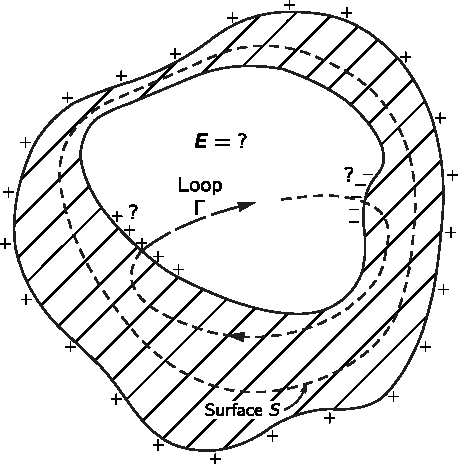
\includegraphics[width=0.8\linewidth]{fyz_fig196.pdf}
    \caption{Jaké pole je v prázdné dutině ve vodiči při jakémkoliv tvaru vodiče a dutiny?}
    \label{fyz:fig196}
  \end{figure}
  Křivkový integrál pole \(\vec{E}\) po každé uzavřené křivce je však v elektrostatickém poli 
  roven nule. Z toho vyplývá, že uvnitř prázdné dutiny nemohou existovat žádná pole ani žádné 
  náboje na jejím povrchu.
  
  Měli bychom si pečlivě všimnout důležité výhrady, kterou jsme uvedli. Vždy jsme říkali 
  „uvnitř prázdné“ dutiny. Umístí-li se totiž nějaké náboje do některých pevných poloh v 
  dutině, ať už v izolantu, nebo na malém vodiči izolovaném od hlavního vodivého tělesa, pak se 
  v dutině mohou objevit pole. Ale pak už to není „prázdná“ dutina.
  
  Ukázali jsme, že je-li dutina úplně obklopena vodičem, žádné statické rozdělení nábojů mimo 
  ni nikdy nemůže vytvořit pole v jejím nitru. Tím se vysvětluje princip „stínění“ elektrického 
  zařízení, které je uloženo v kovovém obalu. Stejné úvahy můžeme použít i v důkazu, že žádné 
  statické rozdělení nábojů uvnitř uzavřeného vodiče nemůže vytvořit nějaká pole ve vnějším 
  prostoru. Stínění funguje v obou směrech. V elektrostatice - ne však při proměnných polích - 
  pole na obou stranách uzavřené vodivé plochy jsou úplně nezávislá.
  
  \emph{Nyní chápeme, proč bylo možné prověřit Coulombův zákon s tak velkou přesností. Tvar 
  duté schránky je bezvýznamný. Nemusí být kulový, mohla by to být krychle. Je-li Gaussův zákon 
  přesný, je pole uvnitř vždy nulové. Teď také chápeme, proč je bezpečné sedět uvnitř 
  vysokonapěťové elektrody megavoltového van de Graaffova generátoru bez obavy ze zásahu 
  elektřinou. Umožňuje to Gaussův zákon.}

%----------------------- Elektrické pole v různých případech -------------------------------------
\section{Elektrické pole v různých případech}\label{fyz:IIchapVsecX}
  Tato kapitola popisuje průběh elektrického pole v řade různých případů. Poskytne určitou 
  informaci o chování elektrického pole a popíše některé z matematických metod používaných pro 
  výpočet tohoto pole.
  
  Nejdříve poukážeme na to, že z matematického hlediska spočívá celá úloha v řešení dvou 
  Maxwellových rovnic pro elektrostatiku:
  \begin{align}
    \nabla\cdot\vec{E}  &= \dfrac{\varrho}{\epsilon_0}  \label{fyz:eq_fey_001} \\
    \nabla\times\vec{E} &= 0.                           \label{fyz:eq_fey_002}
  \end{align}
  
  Ve skutečnosti můžeme obě zkombinovat do jediné rovnice. Z druhé rovnice přímo vidíme, že pole 
  můžeme vyjádřit jako gradient skaláru (viz článek \ref{fyz:IIchapIIIsecVI}):
  \begin{equation}\label{fyz:eq_fey_003}
    \vec{E} = - \nabla\varphi.
  \end{equation}
  Chceme-li, můžeme konkrétní elektrické pole popsat pomocí jeho potenciálu \(\varphi\). Po 
  dosazení do vztahu (\ref{fyz:eq_fey_003}) do rovnice (\ref{fyz:eq_fey_001}) dostaneme 
  diferenciální rovnici, kterou musí splňovat:
  \begin{equation}\label{fyz:eq_fey_004}
  \nabla\cdot\nabla\varphi = - \dfrac{\varrho}{\epsilon_0}.
  \end{equation}
  Divergence gradientu \(\varphi\) je totéž, jako operátor \(\nabla^2\) působící na \(\varphi\), 
  tedy
  \begin{equation}\label{fyz:eq_fey_005}
  \nabla\cdot\nabla\varphi = \nabla^2\varphi 
    = \ppder{\varphi}{x} + \ppder{\varphi}{y} + \ppder{\varphi}{z},
  \end{equation}
  takže rovnici (\ref{fyz:eq_fey_004}) můžeme napsat ve tvaru
  \begin{equation}\label{fyz:eq_fey_006}
  \nabla^2\varphi = - \dfrac{\varrho}{\epsilon_0}.
  \end{equation}
  Operátor \(\nabla^2\) se nazývá \textbf{Laplaceův operátor} a rovnice (\ref{fyz:eq_fey_006}) je 
  \textbf{Poissonova rovnice}. Z matematického hlediska není celá elektrostatika ničím jiným než 
  zkoumáním a řešením této jediné rovnice (\ref{fyz:eq_fey_006}). Jakmile se jejím řešením 
  dostane \(\varphi\), lze \(\vec{E}\) ihned najít ze vztahu (\ref{fyz:eq_fey_003}).
  
  Nejdříve vezměme speciální třídu úloh, ve které je \(\varphi\) dáno jako funkce souřadnic \(x, 
  y, z\). Tehdy je úloha téměř triviální, neboť řešení rovnice (\ref{fyz:eq_fey_006}) pro obecný 
  případ tohoto druhu již známe. Ukázali jsme, že známe-li v každém bodě \(\varrho\), je 
  potenciál v bodě (1)
  \begin{equation}\label{fyz:eq_fey_007}
  \varphi(1) = \int{\dfrac{\varrho(2)}{4\pi\varepsilon_0r_{12}}}\dd{V_2},
  \end{equation}
  kde \(\varrho(2)\) je hustota náboje, \(\dd{V_2}\) je objemový element v bodě (2) a \(r_{12}\) je
  vzdálenost mezi body (1) a (2). Řešení diferenciální rovnice (\ref{fyz:eq_fey_006}) je redukováno
  na integrováním prostoru. Je třeba si zvláště všimnout řešení (\ref{fyz:eq_fey_007}), neboť ve
  fyzice je mnoho situací, jež vedou k rovnicím majícím tvar
  \begin{equation}\label{fyz:eq_fey_008}
  \nabla^2(\text{něco}) = (\text{něco jiného}).
  \end{equation}
  a výraz (\ref{fyz:eq_fey_007}) představuje prototyp řešení pro každou z těchto úloh.
  
  Jsou-li polohy všech bodů známé, výpočet elektrostatického poleje zcela jednoduchý. Ukážeme si to
  na následujících příkladech.

\section{Elektrický dipól}\label{fyz:IIchapVsecXI}
  Vezměme nejdříve dva bodové náboje, stejně velké a opačných znamének, ve vzájemné vzdálenosti
  \(d\). Nechť osa \(z\) prochází náboji a počátek souřadnicové soustavy položme do středu mezi oba
  náboje (obr. \ref{fyz:fig197}). Pak podle (\ref{fyz:fey_eq_elstat24}) je potenciál obou nábojů
  \begin{align}
    \varphi(x,y,z) 
      &= \frac{1}{4\pi\varepsilon_0}
         \left(\dfrac{q}{\sqrt{(z -\frac{d}{2})^2+x^2+y^2}} + \right.    \nonumber \\         
      &+ \left.\dfrac{-q}{\sqrt{(z+\frac{d}{2})^2+x^2+y^2}}\right).      \label{fyz:eq_fey_009}
  \end{align}
  \begin{figure}[ht!] %\ref{fyz:fig197}
    \centering
    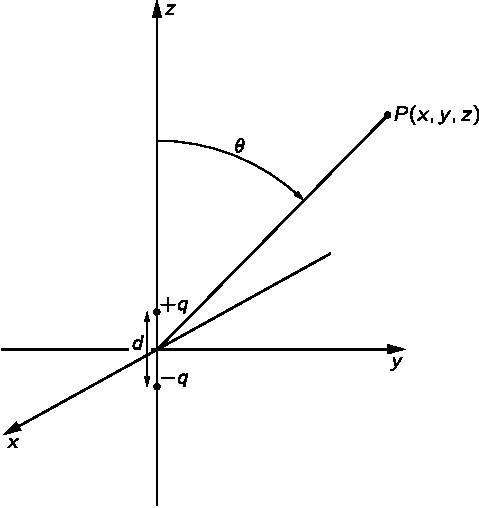
\includegraphics[width=0.7\linewidth]{fyz_fig197.pdf}
    \caption{Dipól: dva náboje \(+q\) a \(-q\) ve vzájemné vzdálenosti \(d\)}
    \label{fyz:fig197}
  \end{figure}
  \emph{Dipólovou anténu} je často možné aproximovat dvěma náboji s malou vzájemnou vzdáleností -
  nezkoumáme-li pole v těsné blízkosti antény. (Obvykle se zajímáme o antény s pohybujícími se
  náboji; potom rovnice elektrostatiky vlastně neplatí, ale pro některé účely jsou vhodným
  přiblížením.)
  
  Důležitější jsou snad \emph{atomové dipóly}. Existuje-li v nějaké látce elektrické pole, působí na
  elektrony opačnou silou než na protony a navzájem je posune. Jak si vzpomínáte, ve vodiči se
  některé z elektronů přesunou k jeho povrchu a pole uvnitř je nulové. V izolantu se elektrony
  nemohou přemístit příliš daleko; přitažlivou silou jádra jsou taženy zpět. Trochu se však posunou.
  Ačkoli atom nebo molekula zůstávají v elektrickém poli neutrální, dochází k velmi jemnému
  rozdělení jejich kladných a záporných nábojů a stanou se mikroskopickými dipóly. Zajímáme-li se o
  pole těchto atomových dipólů v okolí těles s obvyklými rozměry, obyčejně půjde o vzdálenosti,
  které jsou velké ve srovnání se vzdáleností mezi náboji tvořícími páry.
  
  V některých molekulách jsou náboje trochu separovány i bez působení vnějších polí. Je to způsobeno
  tvarem molekuly. Například v \emph{molekule vody} je záporný náboj na atomu kyslíku a kladný náboj
  na každém z obou vodíkových atomů, které však nejsou umístěny souměrně, ale tak, jako na obr.
  \ref{fyz:fig160}. Ačkoliv je náboj celé molekuly roven nule, existuje v ní trochu více záporného
  náboje na jedné straně a trochu více kladného náboje na straně druhé. Toto uspořádání není zajisté
  tak jednoduché jako v případě dvou bodových nábojů, ale díváme-li se na něj z dostatečné
  vzdálenosti, působí jako dipól. Jak uvidíme trochu později, pole ve velkých vzdálenostech není
  citlivé na jemné detaily.

  \begin{figure}[ht!] % \ref{fyz:fig160}
    \centering
    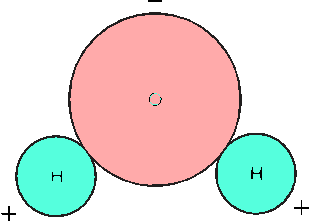
\includegraphics[width=0.4\linewidth]{fyz_fig160.pdf}
    \caption{Molekula vody \(H_20\). Atomy vodíku mají trochu méně z elektronového oblaku než 
      je jejich podíl na jeho vytvoření, zatímco kyslík má trochu více.}
    \label{fyz:fig160}
  \end{figure} 
  Nyní se podívejme na pole dvou opačných nábojů, mezi nimiž je malá vzdálenost \(d\). Je-li \(d\)
  rovno nule, posunou se oba náboje do jednoho místa, oba potenciály se vyruší a žádné pole nebude
  existovat. Jakmile náboje přesně nesplývají, můžeme dostat dobrou aproximaci potenciálu tím, že
  rozvineme členy ve výrazu (\ref{fyz:eq_fey_009}) do mocninné řady podle malé veličiny \(d\)
  (použijeme binomický rozvoj). Zachováme-li členy pouze do prvního řádu \(d\) můžeme psát  
  \begin{equation}\label{fyz:eq_fey_010}
    \left(z-\dfrac{d}{2}\right)^2\approx z^2 - zd.
  \end{equation}
  Je výhodné zavést označení
  \begin{equation}\label{fyz:eq_fey_011}
    x^2 + y^2 + z^2 = r^2.
  \end{equation}
  Potom
  \begin{equation}\label{fyz:eq_fey_012}
    \left(z-\dfrac{d}{2}\right)^2 + x^2 + y^2 \approx r^2 - zd 
      = r^2\left(1 - \dfrac{zd}{r^2}\right) 
  \end{equation}
  a 
  \begin{align}\label{fyz:eq_fey_013}
     \frac{1}{\sqrt{\left(z-\dfrac{d}{2}\right)^2 + x^2 + y^2}}       
    &\approx 
     \frac{1}{\sqrt{r^2\left[1-\left(\dfrac{zd}{r^2}\right)\right]}}   \approx   \nonumber \\
    &\approx 
     \frac{1}{r}\left(1-\frac{zd}{r^2}\right)^{-\frac{1}{2}}. 
  \end{align}
  Rozvineme-li opět výraz \(\left(1-\dfrac{zd}{r^2}\right)^{-\frac{1}{2}}\) do binomické 
  řady\footnote{\((1+\alpha)^{\frac{1}{2}} = 1 - \frac{1}{2}\alpha + \frac{3}{8}\alpha^2 - 
  \frac{15}{48}\alpha^3 + \ldots\)} a zanedbáme členy s mocninami \(d\) vyššími než \(2\), 
  dostaneme výraz
  \begin{equation}\label{fyz:eq_fey_014}
    \frac{1}{r}\left(1+\frac{1}{2}\frac{zd}{r^2}\right). 
  \end{equation}
  Podobně
  \begin{equation}\label{fyz:eq_fey_015}
    \frac{1}{\sqrt{\left(z+\dfrac{d}{2}\right)^2 + x^2 + y^2}}      \approx 
    \frac{1}{r}\left(1-\frac{1}{2}\frac{zd}{r^2}\right). 
  \end{equation}
  Z rozdílu těchto dvou členů vyplývá vztah pro potenciál:
  \begin{equation}\label{fyz:eq_fey_016}
    \varphi(x,y,z) = \dfrac{1}{4\pi\varepsilon_0}\dfrac{z}{r^3}qd
  \end{equation}
  
  \begin{figure}[ht!] % \ref{fyz:fig198}
    \centering
    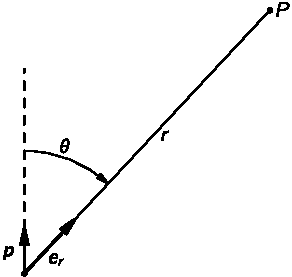
\includegraphics[width=0.5\linewidth]{fyz_fig198.pdf}
    \caption{Vektorová symbolika pro dipól: \(\vec{p} = (0, 0, p)\), \(\vec{r} = (x, 0, z)\), 
             \(\cos\vartheta = \frac{z}{r}\), \(\sin\vartheta = \frac{x}{r}\)}
    \label{fyz:fig198}
  \end{figure}
  Potenciál a tedy i pole jako jeho derivace jsou přímo úměrné veličině \(qd\), tj. součinu
  velikosti každého z nábojů a vzdálenosti mezi nimi. Tento součin je definován jako
  \textbf{elektrický dipólový moment obou nábojů}, pro nějž budeme používat symbol \(p\). (Neplést s
  hybností!):
  \begin{equation}\label{fyz:eq_fey_017}
    p = qd.
  \end{equation}
  Vztah (\ref{fyz:eq_fey_016}) je možné napsat i takto
  \begin{equation}\label{fyz:eq_fey_018}
    \varphi(x,y,z) = \dfrac{1}{4\pi\varepsilon_0}\dfrac{p\cos\vartheta}{r^2},
  \end{equation}
  protože \(\dfrac{z}{r} = \cos\vartheta\), kde \(\vartheta\) je úhel mezi osou dipólu a polohovým
  vektorem bodu \((x, y, z)\) - viz obr. \ref{fyz:fig197}. Pro daný směr vzhledem k ose klesá
  potenciál dipólu jako \(\dfrac{1}{r^2}\) (zatímco pro bodový náboj klesá jako \(\dfrac{1}{r})\).
  Elektrické pole dipólu pak bude klesat jako \(\dfrac{1}{r^3})\).

  Náš vzorec můžeme přepsat na \emph{vektorový tvar}, definujeme-li \(\vec{p}\) jako vektor, který
  má velikost \(p\) a směřuje rovnoběžné s osou dipólu od \(q_-\) do \(q_+\). Pak
   \begin{equation}\label{fyz:eq_fey_019}
    p\cos\vartheta = \vec{p}\cdot\vec{e}_r.
  \end{equation}
  kde \(\vec{e}_r\) je \emph{jednotkový vektor} ve směru polohového vektoru (obr. \ref{fyz:fig197}).
  Kromě toho bod \((x, y, z)\) můžeme určit polohovým vektorem \(\vec{r}\). Pak \textbf{potenciál
  dipólu}:
  \begin{equation}\label{fyz:eq_fey_020}
    \varphi(x,y,z) = \dfrac{1}{4\pi\varepsilon_0}\dfrac{\vec{p}\cdot\vec{e}_r}{r^2}
                   = \dfrac{1}{4\pi\varepsilon_0}\dfrac{\vec{p}\cdot\vec{r}}{r^3}.
  \end{equation}
  Tento vzorec platí pro dipól s jakoukoliv orientací a polohou, představuje-li \(\vec{r}\) vektor
  směřující od dipólu do bodu, o který se zajímáme.

  Chceme-li určit elektrické pole dipólu, můžeme jej vypočítat jako gradient potenciálu 
  \(\varphi\).

  Například \(z\)-ová složka pole je \(\pder{\varphi}{z}\). Pro dipól orientovaný ve směru osy \(z\)
  tj. konfigurace na obr. \ref{fyz:fig197} můžeme použít vztah (\ref{fyz:eq_fey_016}) a dostaneme
  
  \begin{equation}\label{fyz:eq_fey_021}
  -\pder{\varphi}{z}
     = - \frac{p}{4\pi\varepsilon_0}\pder{}{z}\left(\dfrac{z}{r^3}\right)
     = - \frac{p}{4\pi\varepsilon_0}\left(\frac{1}{r^3}-\dfrac{3z^2}{r^5}\right) 
  \end{equation}
  nebo
  \begin{equation}\label{fyz:eq_fey_022}
    E_z = - \frac{p}{4\pi\varepsilon_0}\left(\dfrac{3\cos^2\vartheta-1}{r^3}\right),
  \end{equation}
  \(x\)-ová a \(y\)-ová složka je vyjádřena takto:
  \begin{equation}\label{fyz:eq_fey_023}
    E_x = - \frac{p}{4\pi\varepsilon_0}\dfrac{3zx}{r^5}, \quad
    E_y = - \frac{p}{4\pi\varepsilon_0}\dfrac{3zy}{r^5}.
  \end{equation}
  Je možné složit obě do jedné složky, směřující kolmo na osu \(z\), kterou budeme nazývat příčná
  složka \(E_\perp\):
  \begin{align}
    E_\perp &= \sqrt{E_x^2 + E_y^2} 
             = - \frac{p}{4\pi\varepsilon_0}\dfrac{3z}{r^5}\sqrt{x^2+y^2} \nonumber \\
    \shortintertext{nebo}
    E_\perp &= - \frac{p}{4\pi\varepsilon_0}\dfrac{3\cos\vartheta\sin\vartheta}{r^3} 
                                                                         \label{fyz:eq_fey_024}
  \end{align}
  Příčná složka \(E_\perp\) leží v rovině \(xy\) a směřuje kolmo k dipólu. Výsledné pole dipólu má
  velikost
  \begin{equation}\label{fyz:eq_fey_025}.
    E = \sqrt{E_z^2 + E_\perp^2} 
  \end{equation}
  
  Pole dipólu se mění nepřímo úměrně třetí mocnině vzdálenosti od dipólu. Na ose je při \(\vartheta=
  0\) dvakrát silnější než při \(\vartheta=\ang{90}\). Při obou těchto speciálních úhlech má pole
  pouze \(z\)-ovou složku, ale s opačným znaménkem (obr. \ref{fyz:fig199}).
  \begin{figure}[ht!]
    \centering
    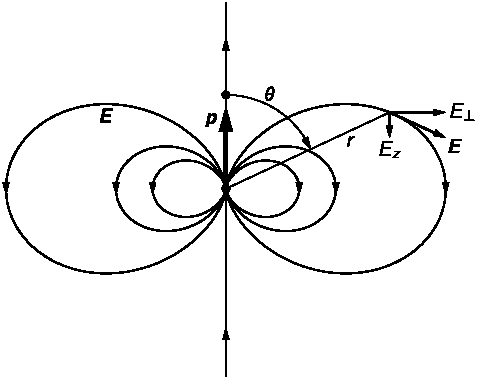
\includegraphics[width=0.7\linewidth]{fyz_fig199.pdf}
    \caption{Elektrické pole dipólu}
    \label{fyz:fig199}
  \end{figure}

\section{Poznámky o vektorových rovnicích}\label{fyz:IIchapVsecXII}
  Zde je namístě udělat obecnou poznámku o vektorové analýze. Ačkoli je možné základní tvrzení
  vyjádřit elegantními rovnicemi v obecném tvaru je při různých výpočtech a analýzách vždy dobré
  zvolit osy nějakým vhodným způsobem. Všimněte si, že když jsme hledali potenciál dipólu, zvolili
  jsme osu \(z\) ve směru dipólu, a ne pod nějakým libovolným úhlem. To nám práci dost zjednodušilo.
  Ale výsledky jsme potom vyjádřili ve vektorovém tvaru, takže už nezávisely na nějaké speciální
  souřadnicové soustavě. Dále můžeme zvolit libovolnou souřadnicovou soustavu, neboť víme, že daný
  vztah platí obecně. Prostě nemá smysl trápit se s obecnou souřadnicovou soustavou s osami
  směřujícími pod nějakým komplikovaným úhlem, když je možné pro danou úlohu zvolit šikovnou
  souřadnicovou soustavu s tím, že výsledek bude stejně vyjádřen jako vektorová rovnice. Všemožně
  tedy využívejte výhodu toho, že vektorové rovnice nezávisí na žádné souřadnicové soustavě.

  Na druhé straně, pokoušíme-li se počítat divergenci vektoru, místo toho, abychom se dívali na
  \(\nabla\cdot\vec{E}\) a přemýšleli, co to je, nezapomeňme, že lze vždy rozepsat jako
  \begin{equation*}
    \pder{E_x}{x} + \pder{E_y}{y} + \pder{E_z}{z}.
  \end{equation*}
  
  Dokážete-li pak vypočítat \(x\)-ovou, \(y\)-ovou a \(z\)-ovou složku elektrického pole a
  derivujete je, dostanete \emph{divergenci}. Často vzniká dojem, že rozepisování složek je cosi
  neohrabaného, jakýsi druh ústupku, že totiž musí vždy existovat nějaký způsob, jak to vše udělat
  pomocí vektorových operátorů. To však často neposkytuje žádnou výhodu. Když se poprvé setkáme s
  nějakou úlohou, je obvykle dobré rozepsat si vše po složkách, abychom se přesvědčili, že rozumíme
  tomu, co se děje. Není nic nešikovného v dosazování čísel do rovnic ani v dosazování derivací za
  fantastické symboly. Naopak, právě s tím je často spojena určitá důmyslnost. Samozřejmě, když
  publikujete článek v odborném časopise, bude vypadat lépe a bude srozumitelnější, dokážete-li vše
  napsat ve vektorovém tvaru. Kromě toho tím ušetříte místo \cite[s.~104]{Feynman02}.
  
\section{Potenciál dipólu jako gradient}\label{fyz:IIchapVsecXIII}
  Rádi bychom poukázali na dost zajímavou vlastnost vztahu (\ref{fyz:eq_fey_020}) pro dipól.
  Potenciál je možné napsat i takto
  \begin{equation}\label{fyz:eq_fey_026}
    \varphi = - \frac{1}{4\pi\varepsilon_0}\vec{p}\cdot\nabla\left(\frac{1}{r}\right).
  \end{equation}
  Vypočítáte-li gradient veličiny \(\frac{1}{r}\), dostanete
  \begin{equation}
    \nabla\left(\frac{1}{r}\right) = -\frac{\vec{r}}{r^3} = -\frac{\vec{e_r}}{r^2},
  \end{equation}
  a vztah (\ref{fyz:eq_fey_026}) je tedy totožný se vztahem (\ref{fyz:eq_fey_020}).

  Jak jsme na to přišli? Jen jsme si vzpomněli, že součinitel \(\dfrac{\vec{e_r}}{r^2}\) se objevil
  i ve vztahu pro pole bodového náboje a toto pole je gradientem potenciálu, který závisí na
  \(\dfrac{1}{r}\).

  Existuje však i fyzikální důvod, že potenciál dipólu lze napsat ve tvaru (\ref{fyz:eq_fey_026}).
  Předpokládejme, že máme bodový náboj v počátku souřadnicové soustavy. Potenciál v bodě \(P\) se
  souřadnicemi \((x,y,z)\) je
  \begin{equation}\label{fyz:eq_fey_027}
    \varphi_0 = \frac{q}{r}.
  \end{equation}
  (Po dobu těchto úvah vynecháme součinitel \(\dfrac{1}{4\pi\varepsilon_0}\); připsat jej můžeme až
  nakonec.) Posuneme- li nyní náboj \(+q\) o vzdálenost \(\Delta z\), potenciál v \(P\) se
  \emph{trochu} změní, řekněme o \(\Delta\varphi_+\).Jakou hodnotu má \(\Delta\varphi_+\)? Takovou,
  o jakou by se potenciál změnil, kdybychom náboj \emph{ponechali} v počátku a posunuli \emph{dolů}
  \(P\) o stejnou vzdálenost \(\Delta z\) (obr. \ref{fyz:fig159}). Tedy
  \begin{figure}[ht!]
    \centering
    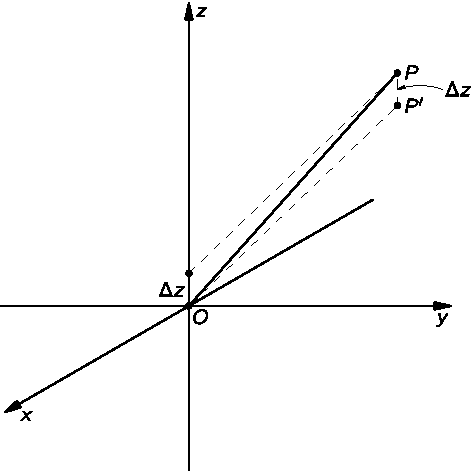
\includegraphics[width=0.6\linewidth]{fyz_fig159.pdf}
    \caption{Potenciál v bodě \(P\) od bodového náboje v poloze \(\Delta z\) nad počátkem
             souřadnicové soustavy je stejný jako potenciál v bodě \(P'\) (posunutém o \(\Delta z\)
             pod \(P\)) od téhož náboje umístěného v počátku}
    \label{fyz:fig159}
  \end{figure}
  \begin{equation}\label{fyz:eq_fey_028}
    \Delta\varphi_+ = \pder{\varphi_0}{z}\Delta z.
  \end{equation}
  kde pod \(\Delta z\) rozumíme totéž jako pod \(\dfrac{d}{2}\). Tak s ohledem na vztah 
  \(\varphi = \frac{q}{r}\) dostáváme, že potenciál souvisící s kladným nábojem je
  \begin{align}
    \varphi_+ &= \frac{q}{r} - 
                 \pder{ }{z}\left(\frac{q}{r}\right)\frac{d}{2}.  \label{fyz:eq_fey_029} \\
    \shortintertext{Ze stejných důvodů můžeme pro potenciál záporného náboje psát}
    \varphi_- &= \frac{-q}{r} + 
                 \pder{ }{z}\left(\frac{-q}{r}\right)\frac{d}{2}. \label{fyz:eq_fey_030} \\
    \shortintertext{Výsledný potenciál je součtem (\ref{fyz:eq_fey_029}) a 
                    (\ref{fyz:eq_fey_030}):}
    \varphi   &= \varphi_+ + \varphi_- = 
                 - \pder{ }{z}\left(\frac{-q}{r}\right)d = 
                 - \pder{ }{z}\left(\frac{1}{r}\right)qd.         \label{fyz:eq_fey_031}
  \end{align}
  Pro jiné orientace dipólu bychom posunuti kladného náboje mohli popsat pomocí vektoru 
  \(\Delta r_+\). Pak bychom vztah (\ref{fyz:eq_fey_029}) napsali takto
  \begin{align}
    \Delta\varphi_+ 
              &= -\nabla\varphi_0\cdot\Delta r_+,                 \label{fyz:eq_fey_032} \\
    \shortintertext{kde je nutné nahradit \(\Delta r\) veličinou \(\dfrac{d}{2}\). Když 
                    dokončíme odvození jako předtím, vztah (\ref{fyz:eq_fey_031}) získá tvar}
    \varphi   &= -\nabla\left(\frac{1}{r}\right)\cdot qd.                      \nonumber \\
    \shortintertext{Je to totéž jako vztah (\ref{fyz:eq_fey_026}), položíme-li 
                    \(q\vec{d}=\vec{p}\) a opět vložíme součinitel 
                    \(\dfrac{1}{4\pi\varepsilon_0}\). Podíváme-li se na to jinak, vidíme, 
                   že potenciál dipólu (vztah \ref{fyz:eq_fey_020}) můžeme zapsat takto}
    \varphi   &= -\vec{p}\cdot\nabla\varphi_0,                    \label{fyz:eq_fey_033}
  \end{align}
  kde \(\varphi_0 = \frac{1}{4\pi\varepsilon_0 r}\) je potenciál jednotkového bodového náboje.
  
  Potenciál známého rozdělení nábojů můžeme vždy vypočítat integrováním. Někdy je však možné ušetřit
  čas pomocí nějakého důvtipného kroku. Například často lze použít princip superpozice. Máme-li
  takové rozdělení nábojů, které je možné popsat jako součet dvou rozdělení, pro které jsou už
  potenciály známé, najdeme požadovaný potenciál snadno prostým sčítáním obou známých potenciálů.
  Jedním takovým příkladem je naše odvození vztahu (\ref{fyz:eq_fey_033}), druhý příklad následuje.
  
  Předpokládejme kulovou plochu s plošným nábojem, jehož rozdělení závisí na kosinu polárního úhlu.
  Takové rozdělení se integruje dost nešikovně. Ale, a to je překvapující, je možné jej analyzovat
  pomocí superpozice. Proto si představte jednu kouli s homogenní \emph{objemovou} hustotou kladného
  náboje a stejně velkou druhou kouli se stejnou objemovou hustotou záporného náboje. Nechť obě
  koule splynou a vytvoří jedinou neutrální, tj. nenabitou kouli. Posune-li se pak kladná koule
  vzhledem k záporné kouli, zůstane těleso jako celek neutrální, ale na jedné straně se objeví malý
  kladný náboj a na opačné straně nějaký záporný náboj, jak to ilustruje obr. \ref{fyz:fig200}.
  Je-li relativní posun obou koulí malý, bude výsledný náboj ekvivalentní plošnému povrchovému
  náboji a jeho plošná hustota bude přímo úměrná kosinu polárního úhlu.
  \begin{figure}[ht!]
    \centering
    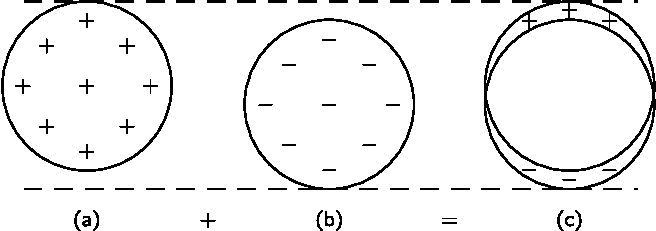
\includegraphics[width=0.7\linewidth]{fyz_fig200.pdf}
    \caption{Dvě objemově rovnoměrně nabité koule pronikající se s malým vzájemným posunutím 
             jsou ekvivalentní s nerovnoměrným rozdělením povrchového náboje}
    \label{fyz:fig200}
  \end{figure}
  
  Potřebujeme-li nyní znát potenciál tohoto rozdělení, nemusíme počítat integrál. Víme, že potenciál
  každé s obou nabitých koulí je v bodech mimo koule stejný jako u bodového náboje. Obě posunuté
  koule jsou jako dva bodové náboje; potenciál je pro ně stejný jako pro dipól.
  
  Tak můžete dokázat, že rozdělení náboje na kulové ploše s poloměrem \(R\) s plošnou hustotou
  \begin{equation}\label{fyz:eq_fey_034}
    \sigma = \sigma_0\cos\vartheta
  \end{equation}
  vytváří na vnější straně kulové plochy pole, které je totožné s polem dipólu s momentem
  \begin{equation}\label{fyz:eq_fey_035}
      p = \frac{4\pi\sigma_0 R^3}{3}.
  \end{equation}      
  Kromě toho lze ukázat, že uvnitř koule je konstantní pole s velikostí
  \begin{equation}\label{fyz:eq_fey_036}
    E = \frac{\sigma_0}{3\varepsilon_0}.
  \end{equation}   
  Je-li \(\vartheta\) úhel odklonu od kladného směru osy \(z\), má elektrické pole uvnitř koule směr
  záporné osy \(z\). Příklad, který jsme právě rozebrali, není tak umělý, jak by se snad zdálo. Opět
  se s ním setkáme V teorii dielektrik.

\section{Dipólové přiblížení pro libovolné rozdělení náboje}\label{fyz:IIchapVsecXIV}
  Pole dipólu se jeví zajímavým a důležitým ještě v jedné situaci. Představte si, že máme těleso se
  složitým rozdělením náboje, řekněme molekulu vody (obr. \ref{fyz:fig160}), a zajímá nás pole pouze
  daleko od něj. Ukážeme, že lze najít poměrně jednoduchý výraz pro pole, platící na vzdálenostech,
  jež jsou vzhledem k rozměrům tělesa velké.

  \begin{figure}[ht!]   %\ref{fyz:fig158}
    \centering
    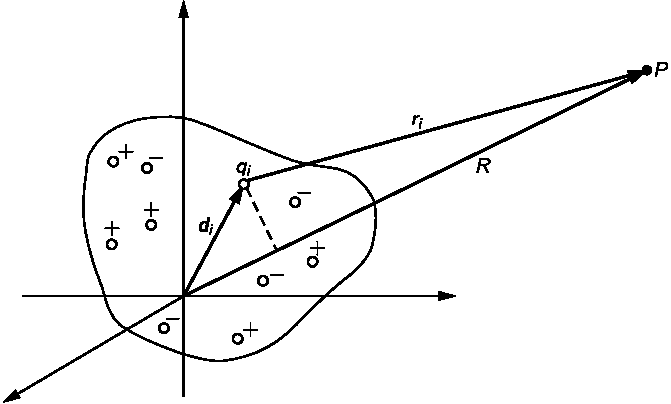
\includegraphics[width=0.7\linewidth]{fyz_fig158.pdf}
    \caption{Výpočet potenciálu v bodě \(P\) nacházejícím se ve velké vzdálenosti od soustavy 
             nábojů \cite[s.~107]{Feynman02}}
    \label{fyz:fig158}
  \end{figure}
  
  Naše těleso můžeme považovat za soubor nábojů \(q_i\), rozmístěných v určité vymezené oblasti, jak
  to znázorňuje obr. \ref{fyz:fig158} (Později můžeme, budeme-li chtít, nahradit \(q_i\) veličinou
  od \(\varrho\dd{V}\).). Nechť se každý náboj \(q_i\), nachází v poloze \(\vec{d}_i\) vzhledem k
  počátku souřadnicové soustavy,jenž byl zvolen někde ve středu skupiny nábojů. Čemu je roven
  potenciál v bodě \(P\) nacházejícím se v poloze \(\vec{R}\) vzhledem k počátku, přičemž délka
  \(\vec{R}\) je mnohem větší než délka největšího posunutí \(\vec{d}\)? Potenciál pocházející od
  celého souboru je
  \begin{equation}\label{fyz:eq267}
    \varphi = \dfrac{1}{4\pi\varepsilon_0}\sum_i\dfrac{q_i}{r_i}
  \end{equation}
  kde \(r_i\) je vzdálenost od \(P\) k náboji \(q_i\), (délka vektoru \(\vec{R}-\vec{d}_i\)). Je-li
  nyní vzdálenost nábojů od \(P\), tj. bodu pozorování, velmi velká, je možné každou z hodnot
  \(r_i\) aproximovat hodnotou \(R\). Každý člen sumy pak bude roven \(\frac{q_i}{R}\) a
  \(\frac{1}{R}\) můžeme vyjmout před znak součtu jako součinitel. Dostaneme jednoduchý výsledek, že
  \begin{equation}\label{fyz:eq268}
   \varphi = \dfrac{1}{4\pi\varepsilon_0}\dfrac{1}{R}\sum_i q_i, 
           = \dfrac{Q}{4\pi\varepsilon_0R}
  \end{equation}
  kde \(Q\) je celkový náboj tělesa. Tak jsme zjistili, že pro body, jež se nacházejí dostatečně 
  daleko od jakéhokoliv nabitého tělesa, se toto těleso jeví jako bodový náboj. Ovšem tento 
  výsledek není příliš překvapující. 
  
  Ale co když jde o stejná množství kladného a záporného náboje? Celkový náboj je pak roven nule.
  Toto není neobyčejný případ; ve skutečnosti, jak víme, bývají tělesa obvykle neutrální. Molekula
  vody je neutrální, ale náboje v ní se nenacházejí všechny v jednom bodě, takže jsme-li dost
  blízko, měli bychom pozorovat nějaké účinky oddělených nábojů. Pro potenciál libovolného rozdělení
  náboje v neutrálním tělese potřebujeme tedy lepší aproximaci, než je (\ref{fyz:eq268}). Výraz
  (\ref{fyz:eq267}) je ještě přesný, ale už nemůžeme klást \(r_i = R\). Potřebujeme vyjádřit
  \(r_i\), přesněji. Je-li bod \(P\) ve velké vzdálenosti, bude se \(r_i\) lišit od \(R\) ve
  výborném přiblížení o průmět \(\vec{d}\) na \(\vec{R}\), jak se můžete přesvědčit z obr.
  \ref{fyz:fig158}. (Uvědomme si, že \(P\) je ve skutečnosti o mnoho dál, než je vidět na obrázku.)
  Jinými slovy, je-li \(\vec{e}_r\), jednotkový vektor ve směru \(\vec{R}\), je potom naše
  následující přiblížení k \(r_i\)
  \begin{align}
   r_i &\approx R - \vec{d}_i\cdot\vec{e}_r.  \label{fyz:eq269a} \\
   \shortintertext{Ve skutečnosti potřebujeme \(1/r_i\), což můžeme v naší aproximaci zapsat jako}
   \frac{1}{r_i} 
       &\approx \frac{1}{R}\left(1 +\frac{\vec{d}_i\cdot\vec{e}_r}{R}\right), \label{fyz:eq269b}
  \end{align}
  protože \(d\ll R\). Po dosazení tohoto výrazu do (\ref{fyz:eq269b}) dostaneme, že potenciál je
  \begin{equation}\label{fyz:eq270}
   \varphi = \dfrac{1}{4\pi\varepsilon_0}
             \left(\dfrac{Q}{R} + \sum_i q_i\frac{\vec{d}_i\cdot\vec{e}_r}{R^2} + \ldots\right).
  \end{equation}
  Tři tečky označují členy s vyšším řádem veličiny \(\frac{d}{R}\), které jsme zanedbali. Tyto,
  jakož i ty členy, které jsme vypsali, představují za sebou následující členy v Taylorově rozvoji
  \(\frac{1}{r_i}\), kolem hodnoty \(\frac{1}{R}\), uspořádané podle mocnin \(\frac{d_i}{R}\). 
  
  První člen v (\ref{fyz:eq270}) je totožný s tím, který jsme dostali předtím; vypadne, je-li těleso
  neutrální. Druhý člen závisí na \(\frac{1}{R^2}\) tak jako v případě dipólu. Ve skutečnosti,
  \emph{definujeme-li}
  \begin{equation}\label{fyz:eq271}
    \vec{p} = \sum_i q_i\vec{d}_i,
  \end{equation}
  jako vlastnost rozdělení náboje, druhý člen ve výrazu (\ref{fyz:eq270}) pro potenciál 
  \begin{equation}\label{fyz:eq272}
   \varphi = \dfrac{1}{4\pi\varepsilon_0}\frac{\vec{p}\cdot\vec{e}_r}{R^2}.
  \end{equation}
  je \emph{přesně potenciálem dipólu}. Veličina \(\vec{p}\) se nazývá \emph{dipólovým momentem
  rozdělení}. Jde o zobecnění naší dřívější definice a na ni se redukuje ve speciálním případě dvou
  bodových nábojů. 
  
  Dospěli jsme k výsledku, že dostatečně daleko od jakéhokoliv seskupení nábojů, které je jako celek
  neutrální, má potenciál charakter potenciálu dipólu. Klesá jako \(\frac{1}{R^2}\) a mění se jako
  \(\cos\vartheta\). Jeho velikost závisí na dipólovém momentu rozdělení náboje. Dipólová pole jsou
  důležitá právě z těchto důvodů, neboť jednoduchý případ páru bodových nábojů je velmi ojedinělý.
 
  Molekula vody má např. dost velký dipólový moment. Elektrická pole, která pocházejí z tohoto
  momentu, jsou příčinou některých důležitých vlastností vody. V mnohých molekulách, například
  \ce{CO2}, je v důsledku jejich souměrnosti dipólový moment nulový. Pro ně bychom měli rozvoj
  vypracovat přesněji a do výrazu pro potenciál zahrnout další člen, který klesá jako
  \(\frac{1}{R^3}\) a který se nazývá \emph{kvadrupólovým potenciálem}. O takových případech budeme
  hovořit později.
  
\section{Pole nabitých vodičů}\label{fyz:IIchapVsecXV}
  Tím jsme probrali příklady situací, v nichž známe rozdělení náboje od začátku. Šlo o úlohu bez
  vážných komplikací, vyžadující přinejhorším několik integrování. Nyní se pustíme do docela nové
  úlohy - určit pole v okolí nabitých vodičů.
  
  Předpokládejme, že na libovolný vodič je vložen celkový náboj \(Q\). Nyní nebudeme schopni přesně
  říci, kde jmenovitě se náboje nacházejí. Jsou nějakým způsobem rozloženy na povrchu. Jak se můžeme
  dozvědět, jak se náboje na povrchu rozdělily? Musí se rozdělit tak, aby potenciál na povrchu byl
  konstantní. Kdyby totiž neměl celý povrch stejný potenciál, existovalo by uvnitř vodiče elektrické
  pole a dokud by nevymizelo, nepřestaly by se náboje pohybovat. Obecnou úlohu tohoto druhu můžeme
  řešit následujícím způsobem. Odhadneme rozdělení náboje a vypočítáme jeho potenciál. Ukáže-li se,
  že je všude na povrchu konstantní, je úloha vyřešena. Není-li povrch ekvipotenciální, neuhádli
  jsme rozdělení nábojů správně a musíme hádat znovu - s nadějí, že budeme mít přesnější odhad. Tak
  je možné pokračovat do nekonečna, nejsme-li v postupných odhadech náležitě šikovní.
  
  Otázka, jak uhádnout rozdělení, je matematicky těžká. Příroda na to má, samozřejmě, čas, náboje se
  strkají a tahají, dokud nejsou všechny navzájem vyvážené. Když se však my pokoušíme takto řešit
  tuto úlohu, zabírá nám každý pokus tolik času, že taková metoda je velmi zdlouhavá. V případě
  libovolného souboru vodičů a nábojů může jít o velmi složitou úlohu, kterou nelze obecně řešit bez
  dosti pracných numerických metod. Takové numerické výpočty se v současnosti dají do počítače,
  který práci udělá za nás, je pouze nutné mu „říci“ jak při ní postupovat.
  
  Na druhé straně, existuje mnoho jednodušších praktických případů, v nichž by bylo užitečné vědět,
  jak najít řešení nějakou přímější metodou - bez psaní programu pro počítač. Naštěstí existuje
  nemálo případů, kde je možné odpověď přímo vytáhnout z přírody nějakým trikem. První trik, který
  popíšeme, využívá řešení, která jsme už získali pro situace, kdy náboje zaujímaly dané polohy.
  
\section{Metoda elektrostatického zobrazení}\label{fyz:IIchapVsecXVI}
  Například jsme vypočítali pole dvou bodových nábojů. Obrázek \ref{fyz:fig161} ukazuje některé ze
  siločar a ekvipotenciálních ploch, jež jsme získali výpočty v kapitole \ref{fyz:IIchapIVsecVIII}.
  Uvažujme nyní ekvipotenciální plochu označenou \(A\). Představte si, že bychom vytvarovali nějaký
  tenký kovový plech tak, aby byl přesně shodný s touto plochou. Umístíme-li jej přímo na plochu a
  jeho potenciál upravíme na příslušnou hodnotu, nikdo se nikdy nedoví, že je tam, protože se tím
  nic nezměnilo.

  \begin{figure}[ht!]  %\ref{fyz:fig161}
    \centering
    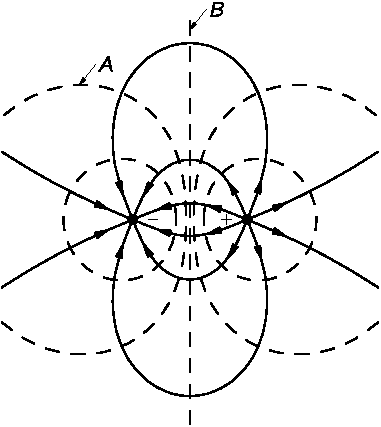
\includegraphics[width=0.7\linewidth]{fyz_fig161.pdf}
    \caption{Siločáry a ekvipotenciální plochy pro dva bodové náboje
             (\cite[s.~110]{Feynman02})}
    \label{fyz:fig161}
  \end{figure}
    
  Ale pozor! Ve skutečnosti jsme vyřešili novou úlohu. Máme situaci, v níž se povrch zakřiveného
  vodiče s daným potenciálem nachází v blízkosti bodového náboje. Uzavírá-li se kovový plech, který
  jsme umístili na ekvipotenciální plochu, sám do sebe (nebo v praxi se táhne dostatečně daleko),
  máme situaci, kterou jsme rozebírali v článku \ref{fyz:IIchapVsecIX}, kdy je prostor rozdělen na
  dvě oblasti - jednu uvnitř a druhou vně uzavřené vodivé plochy. Tam jsme zjistili, že pole v obou
  oblastech jedno na druhém vůbec nezávisí. Na vnější straně našeho zakřiveného vodiče tedy máme
  tatáž pole bez ohledu na to, co je uvnitř. Dokonce můžeme celé nitro vyplnit vodivou látkou. Tak
  jsme našli pole pro uspořádání znázorněné na obr. \ref{fyz:fig162}. V prostoru mimo vodič je pole
  právě takové jako pro dva bodové náboje, tj. jako na obr. \ref{fyz:fig161}. Uvnitř vodiče je rovno
  nule. Kromě toho je pole v bezprostřední blízkosti vodiče - jak to musí být - kolmé na jeho
  povrch.
  
  Podle toho můžeme pole na obr. \ref{fyz:fig162} vypočítat tak, že vypočteme pole pocházející od
  náboje \(q\) a myšleného bodového náboje - \(q\) nacházejícího se ve vhodném bodě. Bodový náboj,
  kterým za vodivou plochou „zobrazujeme“ existující náboj, se nazývá \emph{zrcadlový náboj}.

  \begin{figure}[ht!]  %\ref{fyz:fig162}
    \centering
    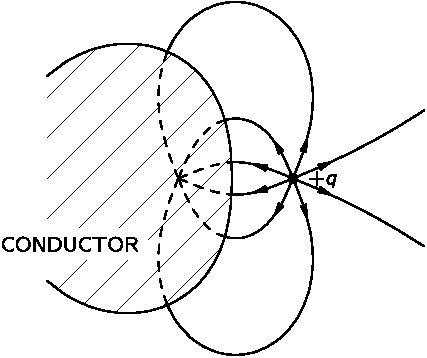
\includegraphics[width=0.7\linewidth]{fyz_fig162.pdf}
    \caption{Pole na vnější straně vodiče, jehož povrch má tvar ekvipotenciální plochy \(A\) na 
             obr. \ref{fyz:fig161}.
             (\cite[s.~110]{Feynman02})}
    \label{fyz:fig162}
  \end{figure}
  
  V knihách můžeme najít dlouhé seznamy řešení pro hyperbolické plochy a další komplikovaně
  vypadající věci a lze se divit, jak někdo dokázal vyřešit úlohu pro tyto hrozné tvary. Byly řešeny
  zpětným postupem. Někdo řešil jednoduchou úlohu s danými náboji. Potom zjistil, že některá
  ekvipotenciální plocha se objevila v novém tvaru a napsal článek o tom, že pole vně tohoto
  konkrétního tvaru je možno popsat určitým způsobem.
  
  \subsection{Bodový náboj v blízkosti vodivé roviny} %\label{fyz:IIchapVsecXVII}
    Jako nejjednodušší aplikaci této metody využijeme rovinnou ekvipotenciální plochu \(B\) na obr.
    \ref{fyz:fig161}. Její pomocí je možné řešit úlohu o náboji v blízkosti vodivé roviny, přičemž
    pouze „vymažeme“ levou polovinu obrázku. Siločáry v našem řešení znázorňuje obr.
    \ref{fyz:fig163}. Všimněme si, že rovina, protože procházela středem mezi oběma náboji, má
    nulový potenciál. Tím jsme tedy řešili úlohu o kladném náboji v blízkosti uzemněné vodivé
    roviny.
    
    Našli jsme celkové pole, ale jak je to s reálnými náboji, které je vytváří? Kromě našeho
    kladného bodového náboje existují i určité indukované záporné náboje na vodivé rovině,
    přitahované naším bodovým nábojem (z velkých vzdáleností). Nyní předpokládejme, že z nějakého
    technického důvodu, nebo z čisté zvědavosti, bychom se rádi dověděli, jak jsou tyto záporné
    náboje na vodivé ploše rozděleny.
    
    \begin{figure}[ht!]  %\ref{fyz:fig163}
      \centering
      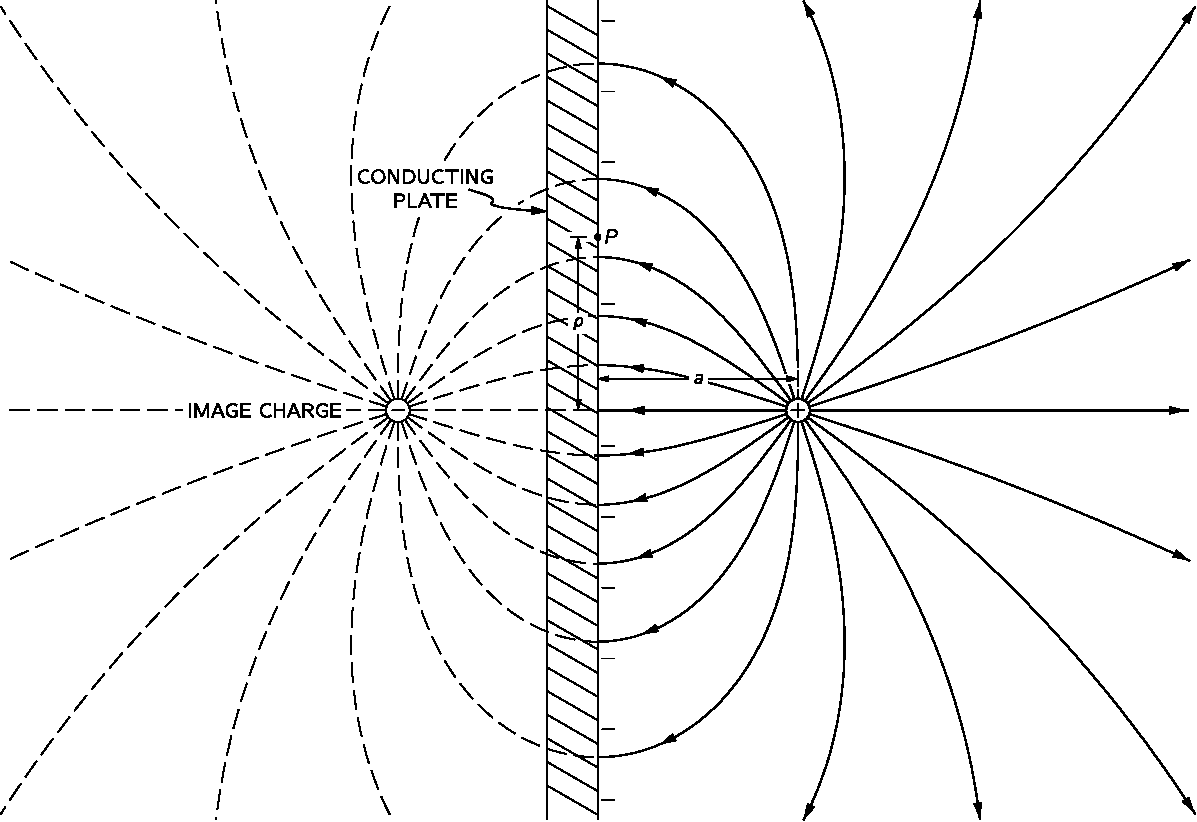
\includegraphics[width=0.9\linewidth]{fyz_fig163.pdf}
      \caption{Pole náboje v blízkosti rovinné vodivé plochy najdeme metodou zrcadlových 
               elektrických nábojů (\cite[s.~111]{Feynman02}).}
      \label{fyz:fig163}
    \end{figure}
    
    Hustotu plošného náboje můžete najít použitím výsledku, k němuž jsme dospěli pomocí Gaussovy
    věty v článku \ref{fyz:IIchapVsecV}. Normálová složka elektrického pole bezprostředně při
    povrchu vodiče je rovna hustotě náboje \(\sigma\) dělené \(\varepsilon_0\). Hustotu náboje v
    jakémkoliv bodě na povrchu vodiče můžeme tedy dostat zpětným postupem z normálové složky
    elektrického pole při povrchu. A tu známe, neboť pole známe všude.
    
    Uvažujme bod Pna povrchu ve vzdálenosti god bodu, který leží přímo protikladnému náboji (obr.
    \ref{fyz:fig163}). V bodě \(P\) je elektrické pole kolmé na povrch a směřuje k němu. Normálová
    složka pole od kladného bodového náboje je
    \begin{equation}\label{fyz:eq287}
     E_{n+} = -\dfrac{1}{4\pi\varepsilon_0}\frac{aq}{(a^2+\varrho^2)^{\frac{3}{2}}}.
    \end{equation}
    K této hodnotě musíme přičíst elektrické pole vytvářené záporným zrcadlovým nábojem. Ten
    zdvojnásobuje normálovou složku (a ruší všechny jiné složky), takže plošná hustota náboje
    \(\sigma\) v každém bodě plochy je
    \begin{equation}\label{fyz:eq288}
     \sigma(\varrho) = \varepsilon_0E(\varrho) = -\frac{2aq}{4\pi(a^2+\varrho^2)^{\frac{3}{2}}}.
    \end{equation} 
    Zajímavý způsob, jak ověřit naše výpočty, spočívá v integrování \(\sigma\) přes celou 
    plochu. Zjistíme, že sumární indukovaný náboj je \(-q\), tak jak má být. 
    
    Můžeme si položit další otázku. Působí na náš bodový náboj nějaká síla? Odpověď: Ano, neboť
    existuje přitahování k zápornému plošnému náboji indukovanému v rovině. Protože nyní víme, jaké 
    jsou plošné náboje (ze vztahu \ref{fyz:eq288}), mohli bychom vypočítat sílu působící na náš 
    kladný náboj integrálem. My už však také víme, že síla na něj působící je přesně taková, jaká 
    by byla se záporným zrcadlovým nábojem místo vodivé desky, protože v obou případech jsou pole v 
    okolí stejná. Bodový náboj je přitahován směrem k desce silou, jejíž velikost tedy je
    \begin{equation}\label{fyz:eq289}
     F = \dfrac{1}{4\pi\varepsilon_0}\frac{q^2}{(2a)^2}.
    \end{equation} 
    Tak jsme našli sílu o mnoho snáze než integrováním přes všechny záporné náboje.
    
  \subsection{Bodový náboj v blízkosti vodivé koule}  %\label{fyz:IIchapVsecXVIII}
    Jaké jiné plochy kromě roviny mají jednoduché řešení? Další nejjednodušší tvar má kulová 
    plocha. Najděme tedy pole v okolí kovové koule, v jejíž blízkosti je bodový náboj (obr. 
    \ref{fyz:fig164}). Musíme hledat takovou jednoduchou fyzikální situaci, v níž bude některá 
    ekvipotenciální hladina kulovou plochou. Poohlédneme-li se po úlohách, které už lidé vyřešili, 
    zjistíme, že existence ekvipotenciální plochy kulového tvaru byla zaznamenána v poli dvou 
    různých bodových nábojů. Zvolíme-li polohu zrcadlového náboje a jeho správnou velikost, 
    dokážeme možná ztotožnit tuto ekvipotenciální plochu s naší koulí. Opravdu toho lze dosáhnout 
    podle následujícího návodu.
    
    Předpokládejme, že chceme, aby ekvipotenciální plocha byla kulovou plochou s poloměrem \(a\), 
    přičemž její střed se nachází ve vzdálenosti \(b\) od náboje \(q\). Umístěme obraz náboje \(q' 
    = -q(a/b)\) na spojnici náboje se středem koule ve vzdálenosti \(a^2/b\) od středu koule. Koule 
    pak bude mít nulový potenciál.
    
    Matematické zdůvodnění je založeno na skutečnosti, že kulová plocha je množinou bodů, jejichž 
    vzdálenosti od dvou pevných bodů jsou ve stálém poměru. Z obr. \ref{fyz:fig164} vyplývá, že 
    potenciál v bodě \(P\) od nábojů \(q\) a \(q'\) je přímo úměrný veličině
    \begin{equation*}
      \dfrac{q}{r_1} + \dfrac{q'}{r_2}.
    \end{equation*}
    Bude tedy roven nule ve všech bodech, pro které
    \begin{equation*}
      \dfrac{q}{r_1} = -\dfrac{q'}{r_2} \quad\text{nebo} \dfrac{r_2}{r_1} = -\dfrac{q'}{q}.
    \end{equation*}
    
    \begin{figure}[ht!]  %\ref{fyz:fig164}
      \centering
      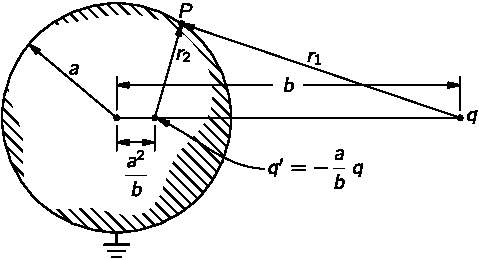
\includegraphics[width=0.8\linewidth]{fyz_fig164.pdf}
      \caption{Bodový náboj \(q\) indukuje na uzemněné vodivé kouli náboje vytvářející stejné pole 
               jako zrcadlový náboj \(q'\) umístěný přesně v ukázaném bodě 
               (\cite[s.~113]{Feynman02}).}
      \label{fyz:fig164}
    \end{figure}
    
    Umístíme-li \(q'\) do vzdálenosti \(a^2/b\) od středu koule, bude mít poloměr \(r_2/r_1\) 
    stálou hodnostu \(a/b\). Je-li potom
    \begin{equation}\label{fyz:eq290}
      \dfrac{r_2}{r_1} = -\dfrac{q'}{q},
    \end{equation}
    povrch koule je ekvipotenciální plochou. Její potenciál je opravdu roven nule. Co se stane, 
    zajímá-li nás koule, která není na nulovém potenciálu? Tak by to bylo pouze tehdy, kdyby její 
    celkový náboj byl náhodou \(q'\). Samozřejmě, je-li uzemněná, musí být náboje na ní indukované 
    rovny právě této hodnotě. Ale co když je izolovaná a nepřivedli jsme na ni žádný náboj? Nebo 
    víme-li, že na ni byl uložen celkový náboj \(Q\)? Nebo pouze, že má nenulový potenciál? Všechny 
    tyto otázky lze snadno zodpovědět. Vždy můžeme přidat bodový náboj \(q''\) do středu koule. 
    Kulová plocha přitom zůstane ekvipotenciální na základě superpozice; změní se pouze hodnota 
    jejího potenciálu. 
    
    Máme-li například vodivou kouli, která je původně nenabitá a od všeho izolovaná a přiblížíme k 
    ní kladný bodový náboj \(q\), zůstane celkový náboj koule nulový. Řešení najdeme 
    pomocí zrcadlového náboje \(q'\) jako předtím, přidáme-li kromě toho do středu koule náboj 
    \(q''\), přičemž
    \begin{equation}\label{fyz:eq291}
      q'' = -q' = \dfrac{a}{b}q,
    \end{equation}
    Pole všude v okolí koule určíme superpozicí polí od \(q\), \(q'\) a \(q''\). Úloha je tak 
    vyřešena.
    
    Nyní se můžeme přesvědčit, že mezi koulí a bodovým nábojem \(q\) bude působit přitažlivá síla. 
    Ta není nulová ani tehdy, když na neutrální kouli není žádný náboj. Z čeho pochází toto 
    přitahování? Přiblížíme-li k vodivé kouli kladný náboj, přitáhne na její přivrácenou stranu 
    záporné náboje, zatímco kladné ponechá na povrchu vzdálené strany. Přitahování zápornými náboji 
    převáží odpuzování kladnými náboji a výsledkem je přitahování. Jeho velikost můžeme najít 
    výpočtem síly působící na \(q\) v poli vytvořeném náboji \(q'\) a \(q''\). Výsledná síla je 
    součtem přitažlivé síly mezi \(q\) a nábojem \(q' = -\dfrac{a}{b}q\), jenž se nachází ve 
    vzdálenosti \(b - (a^2/b)\) od \(q\) a odpudivé síly mezi \(q\) a nábojem \(q'' = 
    \dfrac{a}{b}q\), který je ve vzdálenosti \(b\) od \(q\). 
    
    Ty, které v dětství zaujala krabička s práškem do pečiva, na které byl obrázek krabičky s 
    práškem do pečiva, ... snad zaujme následující úloha. V určité vzdálenosti od sebe se 
    nacházejí dvě koule, jedna s celkovým nábojem \(+Q\) a druhá s celkovým nábojem  \(-Q\) Jaká 
    mezi nimi působí síla? Úlohuje možno řešit pomocí nekonečného počtu zrcadlení. Nejdříve je 
    každá koule aproximována nábojem v jejím středu. Každá z nich má svůj zrcadlový náboj v druhé 
    kouli. Zrcadlové náboje budou mít své zrcadlové náboje atd., atd., atd. Řešení připomíná 
    obrázek na krabičce spráškem do pečiva a konverguje velice rychle.

\section{Kondenzátory, rovnoběžné desky}\label{fyz:IIchapVsecXIX}
  Nyní se budeme zabývat jinou úlohou týkající se vodičů. Uvažujme dvě rovnoběžné kovové 
  desky, jejichž vzájemná vzdálenost je malá ve srovnání s jejich rozměry. Předpokládejme, že jsme
  na desky přivedli stejně velké náboje s opačnými znaménky. Náboje na každé z desek budou 
  přitahovány náboji na druhé desce a rozdělí se rovnoměrně na vnitřním povrchu desek. Plošné
  hustoty nábojů na deskách budou \(+\sigma\), resp. \(-\sigma\) (obr.\ref{fyz:fig165}). Z kapitoly 
  \ref{fyz:IIchapVsecV} víme, že pole mezi deskami je \(\sigma/\varepsilon_0\), a mimo desky je 
  rovno nule. Desky budou mít rozdílné potenciály \(\varphi_1\), a \(\varphi_2\). Je vhodné označit 
  jejich rozdíl písmenem \(U\) a nazvat jej \emph{napětím}:
  \begin{equation}\label{fyz:eq292}
    \varphi_1 - \varphi_2 = U.
  \end{equation}
  
  \begin{figure}[ht!]  %\ref{fyz:fig165}
    \centering
    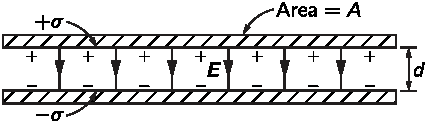
\includegraphics[width=1\linewidth]{fyz_fig165.pdf}
    \caption{Kondenzátor s rovnoběžnými rovinnými elektrodami 
             (\cite[s.~114]{Feynman02}).}
    \label{fyz:fig165}
  \end{figure}
  
  Rozdíl potenciálů je práce připadající na jednotku náboje, jež je spotřebována na přenos malého 
  náboje z jedné desky na druhou, takže
  \begin{equation}\label{fyz:eq293}
    U = Ed = \dfrac{\sigma}{\varepsilon_0}d = \dfrac{d}{\varepsilon_0S}Q.
  \end{equation}
  kde \(\pm Q\) je celkový náboj na každé desce, \(S\) je plošný obsah desek a \(d\) je jejich 
  vzájemná vzdálenost.
  
  Vidíme, že napětí je přímo úměrné náboji. Přímá úměrnost mezi \(U\) a \(Q\) platí pro jakékoliv 
  dva vodiče v prostoru, je-li na jednom z nich kladný a na druhém stejně velký záporný náboj. 
  Rozdíl potenciálů mezi nimi, tj. napětí, je přímo úměrný náboji. (Přitom předpokládáme, že v 
  okolí nejsou jiné náboje.)
  
  Proč platí tato přímá úměrnost? Plyne z principu superpozice. Předpokládejme, že známe řešení pro 
  jednu sadu nábojů a chceme složit dvě taková řešení. Náboje se zdvojnásobí, pole se zdvojnásobí, 
  a zdvojnásobí se tedy i práce konaná při přenosu jednotkového náboje z jednoho bodu do druhého. 
  Proto je rozdíl potenciálů jakýchkoliv dvou bodů přímo úměrný nábojům. Speciálně, rozdíl 
  potenciálů dvou vodičů je přímo úměrný nábojům na nich. Kdosi původně napsal tuto přímou úměrnost 
  obráceně, tj.
  \begin{equation}\label{fyz:eq294}
    Q = CU,
  \end{equation}
  kde \(C\) je konstanta. Tento součinitel přímé úměrnosti se nazývá kapacita a taková soustava 
  dvou vodičů je \textbf{kondenzátor}. V případě našeho kondenzátoru s rovnoběžnými deskami platí
  \begin{equation}\label{fyz:eq295}
    C = \frac{\varepsilon_0d}{S} \quad\text{(rovnoběžné desky)},
  \end{equation}
  
  Tento vzorec není přesný, neboť ve skutečnosti není pole všude mezi deskami homogenní, jak jsme 
  předpokládali. Na okrajích desek pole nekončí najednou, ale odpovídá spíš průběhu,
  jaký znázorňuje obr. \ref{fyz:fig166}.
  
  \begin{figure}[ht!]  %\ref{fyz:fig166}
    \centering
    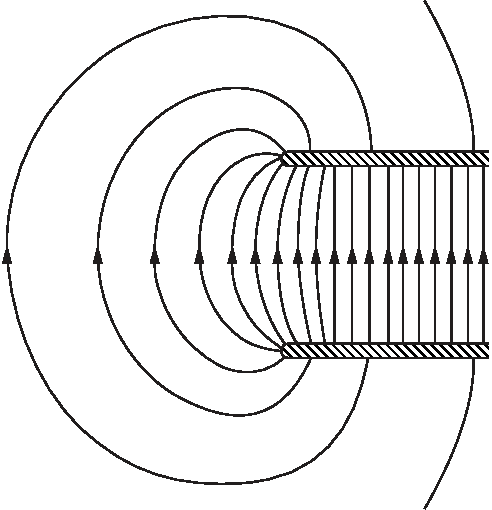
\includegraphics[width=0.7\linewidth]{fyz_fig166.pdf}
    \caption{Elektrické pole v blízkosti okraje dvou rovnoběžných desek
             (\cite[s.~115]{Feynman02}).}
    \label{fyz:fig166}
  \end{figure}

  Celkový náboj není \(σS\), jak jsme předpokládali, ale je třeba provést malou korekci vzhledem k
  okrajovým jevům. Abychom ji dostali, musíme pole vypočítat přesněji a najít, co se děje na
  okrajích. To je složitá matematická úloha. Lze ji však řešit technikou, kterou nebudeme nyní
  popisovat. Výsledky takových výpočtů ukazují, že v blízkosti hran se hustota náboje o něco
  zvětšuje. To znamená, že kapacita desek je trochu větší, než jsme počítali. (Pro kapacitu
  dostaneme velmi dobré přiblížení, použijeme-li vzorec (\ref{fyz:eq295}), ale za \(S\) dosadíme
  plochu, kterou by desky měly, kdybychom jejich rozměry zvětšili o 3/8 vzdálenosti mezi nimi.)
  
  Hovořili jsou pouze o kapacitě dvou vodičů. Někdy se mluví o kapacitě jediného tělesa. Například
  se říká, že kapacita koule s poloměrem \(R\) je \(4π\varepsilon_0R\). Přitom se však rozumí, že druhou
  Elektrodou je koule s nekonečně velkým poloměrem, tj. že je-li náboj \(+Q\) na naší kouli, je
  opačný náboj \(-Q\) na nekonečné kouli. O kapacitách můžeme hovořit i tehdy, když existují tři
  anebo víc vodičů. Diskusi o tom však zatím odložíme.

  Představte si, že chceme mít kondenzátor s velmi velkou kapacitou. Velkou kapacitu bychom mohli
  dostat, kdybychom vzali velmi velkou plochu a velmi malou vzdálenost. Mohli bychom mezi dvě
  hliníkové fólie vložit impregnovaný papír a potom to stočit. (Kdybychom to zapustili do
  plastického pouzdra, dostali bychom typický radiotechnický kondenzátor.) K čemu je to dobré? Hodí
  se to k hromadění náboje. Shromažďujeme-li náboj například na povrchu koule, vzrůstá při nabíjení
  tělesa prudce jeho potenciál. Může dokonce dosáhnout takové hodnoty, že náboj začne jiskrovým
  výbojem unikat do vzduchu. Ale vložíme-li tentýž náboj na kondenzátor s velkou kapacitou, napětí
  na kondenzátoru bude malé.

  V elektronických obvodech je často užitečné mít něco, co může pohlcovat nebo dodávat velká
  množství náboje bez větší změny svého potenciálu. Právě k tomu slouží kondenzátor. V mnoha
  případech se v elektronických přístrojích a v počítačích používá také k tomu, aby na určitou změnu
  náboje reagoval požadovanou změnou napětí. S podobným použitím jsme se seznámili v
  \ref{fyz:IchapXXIII}. kapitole \ref{part:FYZI}. dílu při popisu vlastností rezonančních obvodů.

  Z definice kapacity \(C\) vidíme, že její jednotkou je 1 coulomb/volt. Tato jednotka se nazývá
  \textbf{farad}. Ze vztahu (\ref{fyz:eq295}) dále vidíme, že jednotku veličiny \(\varepsilon_0\) je
  možno vyjádřit jako farad/metr.

  Typické vlastnosti kondenzátorů jsou v rozmezí od jednoho pikofaradu do milifaradů. Malé
  kondenzátory s několika pikofarady se používají ve vysokofrekvenčních ladicích obvodech a kapacity
  až do stovek nebo tisíců mikrofaradů se vyskytují ve vysokonapěťových usměrňovačích. Pár desek s
  plochou jeden centimetr čtvereční a mezerou jeden milimetr má kapacitu zhruba jeden pikofarad.
  
\section{Průraz při vysokém napětí}\label{fyz:IIchapVsecXX}
  Nyní bychom rádi kvalitativně popsali některé charakteristiky polí v okolí vodičů. Nabijeme-li
  vodič, který nemá tvar koule, ale má hrot nebo ostrou hranu, například těleso nakreslené na obr.
  \ref{fyz:fig167}, bude pole v okolí tohoto hrotu mnohem větší než v jiných oblastech. Důvod
  spočívá v tom, kvalitativně řečeno, že náboje mají tendenci se co nejvíc rozestoupit po povrchu
  vodiče a špička hrotu je od většiny povrchu tak daleko, jak je jen to možné. Část nábojů na vodiči
  je tedy odpuzována až ke špičce. Poměrně malé množství náboje na špičce může vést k velké plošné
  hustoty velká hustota náboje znamená silné pole v těsném sousedství.

  \begin{figure}[ht!]  %\ref{fyz:fig167}
    \centering
    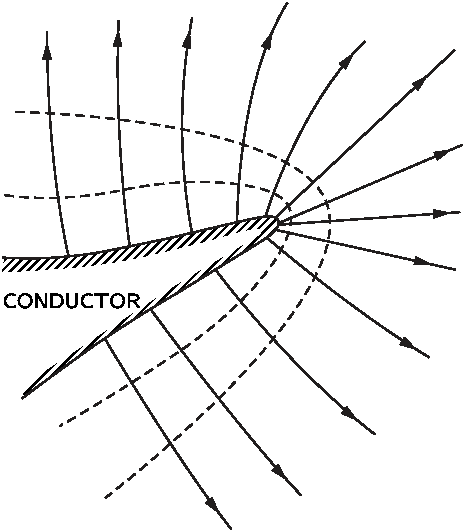
\includegraphics[width=0.7\linewidth]{fyz_fig167.pdf}
    \caption{V blízkosti ostrého hrotu na vodiči je elektrické pole velmi silné
             (\cite[s.~116]{Feynman02}).}
    \label{fyz:fig167}
  \end{figure}

  Jeden způsob, jak se přesvědčit, že nejsilnější pole je v těch místech na vodiči, kde je nejmenší
  poloměr křivosti, spočívá v analýze kombinace dvou koulí, velké a malé, spojených pomocí vodivého
  drátu (obr. \ref{fyz:fig168}).  

  Jde tak o trochu idealizovanou verzi vodivého tělesa z obr. \ref{fyz:fig167}. Drát bude mít malý
  vliv na vnější pole; slouží pouze k tomu, aby se koule udržovaly na stejném potenciálu. Která z
  koulí má na povrchu silnější pole? Má-li koule poloměr \(a\) a nese náboj \(Q\) je její potenciál
  přibližně
  \begin{equation*}
    ϕ_1=\dfrac{1}{4π\varepsilon_0}\dfrac{Q}{a}.
  \end{equation*}
  (Samozřejmě, přítomnost náboje na jedné kouli změní rozdělení náboje na druhé kouli, takže 
  ve skutečnosti ani na jedné z nich nejsou náboje rozděleny s kulovou souměrností. Ale zajímá-li
  vás jen odhad polí, můžeme použít vzorec pro potenciál kulového náboje.) Když menší koule, jejíž
  poloměr je \(b\) nese náboj \(q\) je její potenciál přibližně
  \begin{equation*}
    ϕ_2=\dfrac{1}{4π\varepsilon_0}\dfrac{q}{b}.
  \end{equation*}
  Ale \(ϕ_1=ϕ_2\), takže
  \begin{equation*}
    \dfrac{Q}{a}=\dfrac{q}{b}.
  \end{equation*}
    
  \begin{figure}[ht!]  %\ref{fyz:fig168}
    \centering
    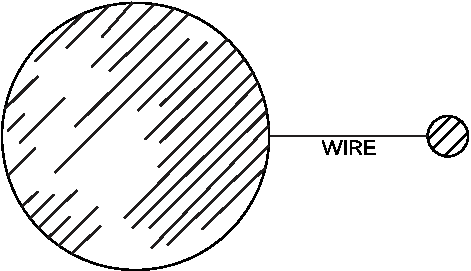
\includegraphics[width=0.7\linewidth]{fyz_fig168.pdf}
    \caption{Pole špičatého tělesa je možné aproximovat polem dvou koulí se stejným potenciálem
             (\cite[s.~116]{Feynman02}).}
    \label{fyz:fig168}
  \end{figure}

  Na druhé straně pole při povrchu (viz vztah \ref{fyz:eq825}) je přímo úměrné
  plošné hustotě náboje, jež je přímo úměrná celkovému náboji dělenému druhou mocninou poloměru.
  Dostáváme, že
  \begin{equation}\label{fyz:eq826}
    \dfrac{E_a}{E_b}=\dfrac{Q/a^2}{q/b^2}=\dfrac{b}{a}.
  \end{equation}
  Z toho vyplývá, že poleje silnější při povrchu malé koule. Pole jsou nepřímo úměrná poloměrům.

  Tento výsledek je velmi důležitý z technického hlediska, neboť je-li elektrické pole příliš silné,
  dojde k průrazu vzduchu. Co se přitom stane? Náboj uvolněný někde ve vzduchu (elektron nebo ion)
  se polem urychlí a je-li pole velmi silné, může náboj dříve, než narazí na jiný atom, nabýt
  rychlost postačující k tomu, aby mohl z atomu vyrazit elektron. Tak vzniká více a více iontů.
  Jejich pohyb vytváří výboj nebo jiskru. Chceme-li těleso nabít na vysoký potenciál a nedopustit
  přitom jeho vybíjení do vzduchu, musíme zabezpečit, aby mělo hladký povrch a neexistovalo tak
  místo, kde by bylo pole abnormálně silné.
  
\section{Emisní mikroskop}\label{fyz:IIchapVsecXXI}  
  Existuje zajímavé využití extrémně silného elektrického pole obklopujícího nějaký ostrý výčnělek
  na nabitém vodiči. Na silných polích vznikajících na ostrém kovovém hrotu je založena
  \emph{činnost emisního mikroskopu}. Je konstruován následujícím způsobem. Velmi jemná jehla s
  hrotem, jehož průměr je asi \num{0.1} mikrometru, se nachází ve středu vakuované skleněné koule
  (obr. \ref{fyz:fig169}). Vnitřní povrch koule je pokrytý tenkou vodivou vrstvou fluorescenční
  látky a mezi jehlu a fluorescenční kryt je vloženo velmi vysoké napětí.

  \begin{figure}[ht!]  %\ref{fyz:fig169}
    \centering
    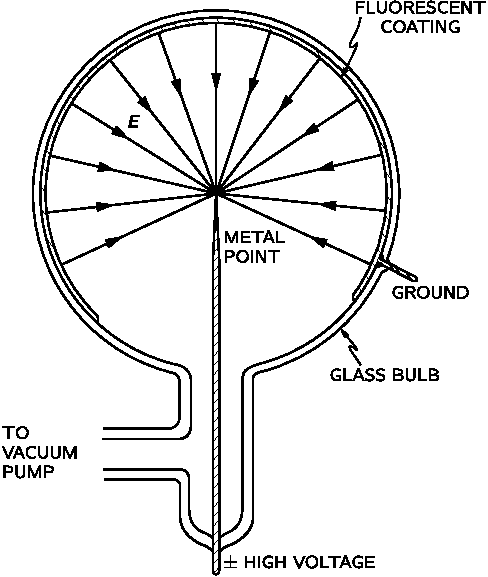
\includegraphics[width=0.7\linewidth]{fyz_fig169.pdf}
    \caption{Emisní mikroskop (\cite[s.~118]{Feynman02}).}
    \label{fyz:fig169}
  \end{figure}

  Nejdříve se podívejme, co se stane, je-li jehla vzhledem k fluorescenčnímu povlaku nabita záporné.
  V okolí jejího hrotu jsou siločáry silně koncentrované. Elektrické pole tam může dosáhnout až 40
  milionů voltů na 1 centimetr. V takových intenzivních polích jsou elektrony vytrhávány z povrchu
  jehly a urychlovány napětím mezi jehlou a fluorescenční vrstvou. Při dopadu na vrstvu vyvolají
  emisi světla právě tak jako v televizní obrazovce.

  \begin{figure}[ht!]  %\ref{fyz:fig936}
    \centering
    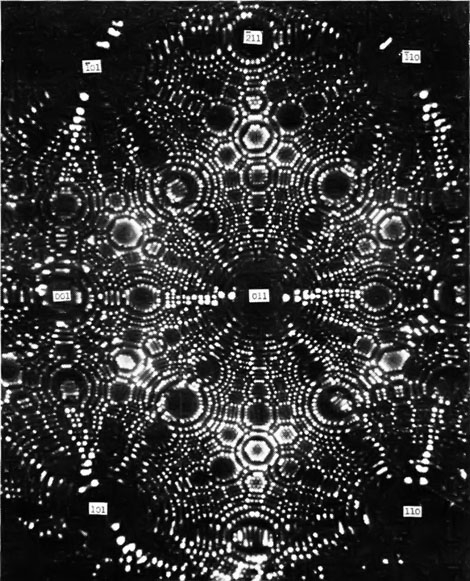
\includegraphics[width=0.7\linewidth]{fyz_fig936.png}
    \caption{Obraz vytvořený emisním mikroskopem (s dovolením Erwina W. Muellera, prof. fyziky na 
            Pennsylvánské státní univerzitě) (\cite[s.~119]{Feynman02}).}
    \label{fyz:fig936}
  \end{figure}

  Elektrony, které přicházejí do daného bodu na fluorescenčním povrchu, jsou s výborným přiblížením
  tytéž, které z jehly vyšly na opačném konci radiální siločáry, neboť se pohybují po siločáře
  jdoucí od hrotu k povrchu. Takovýmto způsobem vidíme na fluorescenčním povrchu určitý obraz špičky
  jehly. Přesněji řečeno, vidíme obraz \textbf{emisivity} povrchu jehly, která je mírou snadnosti, s
  jakou elektrony můžou opustit povrch kovového hrotu. Kdyby rozlišení bylo dostatečně vysoké, byla
  by naděje rozlišit polohy jednotlivých atomů na hrotu jehly. Takové rozlišení však nelze s
  elektrony dosáhnout z následujících důvodů. Zaprvé, existuje kvantově - mechanický ohyb
  elektronových vln, který obraz rozmazává. Zadruhé, v důsledku vnitřního pohybu v kovu mají
  elektrony při výstupu z jehly malou boční počáteční rychlost a tato náhodná příčná složka
  rychlosti také působí určité rozmazání obrazu. Kombinace těchto dvou efektů omezuje rozlišení
  zhruba na \SI{2.5}{\nm}.

  Změníme-li však polaritu a do baňky vpustíme malé množství hélia, lze dosáhnout mnohem většího
  rozlišení. Narazí-li atom hélia na hrot jehly, intenzivní pole v tom místě mu vytrhne elektron, a
  změní jej tím na kladný ion. Héliový ion je pak urychlován po siločáře k fluorescenčnímu stínítku.
  Protože je mnohokrát těžší než elektron, jsou jeho kvantově - mechanické vlnové délky mnohem
  menší. Pokud není teplota příliš vysoká, je účinek tepelných rychlostí také menší než v případě
  elektronů. Rozmazání obrazu bude tedy menší a obraz hrotu mnohem ostřejší. S iontovým emisním
  mikroskopem se podařilo dosáhnout zvětšení až \num{2000000} krát, což je desetkrát lepší než v
  nejlepších elektronových mikroskopech.

  Obrázek \ref{fyz:fig936} je ilustrací výsledků, které byly získány iontovým emisním mikroskopem,
  používajícím wolframovou jehlu. Střed wolframového atomu ionizuje atom hélia s trochu jinou
  pravděpodobností než mezery mezi atomy wolframu. Obrazec skvrn na fluorescenčním stínítku ukazuje
  uspořádání jednotlivých atomů na wolframovém hrotu. To, proč mají skvrny prstencový tvar, můžeme
  pochopit, představíme-li si velkou krabici plnou koulí uložených do pravoúhlé prostorové sítě,
  která představuje uspořádání atomů v kovu. Vyříznete-li z této krabice přibližně kulový výsek,
  uvidíte prstencový obrazec charakteristický pro atomovou strukturu. Iontový emisní mikroskop
  poskytl lidem poprvé v historii možnost uvidět atomy. Když se přitom zváží ještě jednoduchost
  přístroje, jde o pozoruhodný výdobytek.
  
\section{Metody určování elektrostatického pole}\label{fyz:IIchapVsecXXII}
  Tato kapitola je pokračováním našich úvah o charakteristikách elektrických polí v různých
  konkrétních situacích. Nejdříve popíšeme některé ze složitějších metod k řešení úloh s vodiči.
  Neočekáváme, že tyto pokročilejší metody dokážete ihned zvládnout. Už nyní však pro vás bude
  zajímavé získat nějakou představu o tom, jaké úlohy je možno řešit pomocí postupů, o nichž se
  hovoří v pokročilejších kurzech. Potom probereme dva příklady, v nichž není rozdělení náboje ani
  pevné, ani rozloženo na vodiči, aleje určeno nějakým jiným fyzikálním zákonem.

  Jak jsme zjistili v této kapitole, je-li rozdělení nábojů dáno, může být úloha o elektrostatickém
  poli řešena v podstatě snadno´- je třeba pouze vypočítat integrál. Přítomností vodičů však
  vznikají komplikace, neboť rozdělení náboje na vodičích není předem známé; náboj se musí sám
  rozdělit na povrchu vodiče takovým způsobem, aby měl vodič všude stejný potenciál. Takové úlohy
  nelze řešit ani přímo ani snadno. tvaru koulí, rovin atd. Využití zrcadlení, popsané v kapitole
  \ref{fyz:IIchapVsecXVI}, je také příkladem nepřímé metody. Další příklad popíšeme v této kapitole.

  Nepatří-li úloha, která je řešena, do třídy úloh, jejichž řešení jsou konstruovatelná nepřímou
  metodou, jsme nuceni řešit ji přímější metodou. Z matematického hlediska spočívá přímá metoda v
  řešení Laplaceovy rovnice 
  \begin{equation}\label{fyz:eq827}
    \nabla^2\varphi = 0
  \end{equation}
  za podmínky, že \(\varphi\) nabývá vhodné hodnoty na určitých hranicích - na površích vodičů.
  Úlohy, v nichž má řešení diferenciální rovnice pole splňovat určité \emph{okrajové podmínky} se
  nazývají \emph{okrajovými úlohami}. Byly a jsou předmětem intenzivního matematického výzkumu. V
  případě vodičů, majících složité tvary, nejsou na jejich řešení žádné obecné analytické metody. I
  taková jednoduchá úloha, jaká je o nabitém, na obou koncích uzavřeném kovovém válci,
  připomínajícím konzervu je spojena s ohromnými matematickými těžkostmi. Je možné ji řešit pouze
  přibližně, použitím numerických metod. Numerické metody jsou zde jedinými obecnými metodami
  řešení.

  Existuje však několik úloh, v nichž lze rovnice (\ref{fyz:eq827}) řešit přímo. Například úlohu o
  nabitém vodiči tvaru rotačního elipsoidu je možné řešit exaktně pomocí známých speciálních funkcí.
  Necháme-li elipsoid nekonečně zploštit, dostaneme řešení pro případ tenkého kotouče. Podobně lze
  získat řešení pro jehlu, necháme-li elipsoid nekonečně protáhnout. Je však třeba zdůraznit, že
  jedinými přímými metodami s obecnou použitelností jsou numerické metody.

  Okrajové úlohy je možné kromě toho řešit měřením jejich fyzikálních analogií. Laplaceova rovnice
  se vyskytuje v mnoha různých fyzikálních situacích: při stacionárním toku tepla, při bezvírovém
  proudění tekutiny, při průchodu proudu v rozlehlém prostředí a při vychylování pružné membrány.
  Často je proto možné postavit fyzikální model analogický elektrické úloze, již chceme řešit. Její
  řešení je možné najít měřením vhodné analogické veličiny na modelu. Příkladem této metody je
  využití elektrolytické vany k řešení dvojrozměrných úloh v elektrostatice. Je založena na tom, že
  diferenciální rovnice pro potenciál v homogenním vodivém prostředí je stejná jako pro vakuum.

  Je mnoho fyzikálních situací, kdy změny v jednom směru jsou nulové nebo zanedbatelné ve srovnání
  se změnami v druhých dvou směrech. Takové úlohy se nazývají \emph{dvojrozměrné} - pole v nich
  závisí pouze na dvou souřadnicích. Umístíme-li například dlouhý nabitý drát do směru osy z, pro
  body, které nejsou příliš vzdálené od drátu, bude elektrické pole záviset na \(x\) a \(y\), ale ne
  na \(z\), jde o dvojrozměrnou úlohu. Protože ve dvojrozměrné úloze je \(diffp{}{z}=0\), je rovnice
  pro \(\varphi\) ve volném prostoru
  \begin{equation}\label{fyz:eq828}
    \diff[2]{\varphi}{x} + \diff[2]{\varphi}{y} = 0
  \end{equation}
  Protože rovnice se dvěma proměnnými je poměrně jednoduchá, existuje široký rozsah podmínek, za
  kterých ji lze řešit analyticky. Pro takovéto případy existuje vlastně velmi účinná nepřímá
  matematická metoda, zakládající se na jedné větě z teorie funkcí komplexní proměnné, kterou nyní
  popíšeme.

\twocolumn[\section{Dvojrozměrné pole jako funkce komplexní proměnné}\label{fyz:IIchapVsecXXIII}]
  Komplexní proměnná \(\mathfrak{z}\) je definována takto
  \begin{equation*}
    \mathfrak{z} = x + \imath y.
  \end{equation*}
  (Nezaměňujte \(\mathfrak{z}\) se souřadnicí \(z\), kterou z následující úvahy vypouštíme, neboť
  předpokládáme, že na souřadnici \(z\) pole nezávisí.) Každému bodu v rovině \((x, y)\) přísluší
  nějaké komplexní číslo \(\mathfrak{z}\). Můžeme \(\mathfrak{z}\) považovat za jedinou (komplexní)
  proměnnou a její pomocí popsat obvyklé matematické funkce \(F(\mathfrak{z})\). Například
  \begin{align*}
    F(\mathfrak{z}) &= \mathfrak{z}^2     \\
    \shortintertext{nebo}
    F(\mathfrak{z}) &= 1/\mathfrak{z}^3   \\
    \shortintertext{nebo}
    F(\mathfrak{z}) &= \mathfrak{z}\log\mathfrak{z} \\
    \shortintertext{atd.}
  \end{align*}
  Máme-li dané nějaké konkrétní \(F(\mathfrak{z})\), můžeme dosadit \(\mathfrak{z} = x + \imath y\)
  a dostaneme funkci proměnných \(x\) a \(y\) , která má dvě části - reálnou a imaginární. Například
  \begin{equation}\label{fyz:eq829}    
    \mathfrak{z}^2=(x+\imath y)^2=x^2−y^2+2\imath xy.
  \end{equation}
  Každou funkci \(F(\mathfrak{z})\) je možné zapsat jako součet ryze reálné a ryze imaginární části,
  přičemž jedna i druhá jsou funkcemi \(x\) a \(y\)
  \begin{equation}\label{fyz:eq830}    
    F(\mathfrak{z})=U(x,y)+\imath V(x,y)
  \end{equation}
  kde \(U(x, y)\) a \(V(x, y)\) jsou reálné funkce. Tímto způsobem můžeme z každé komplexní funkce
  \(F(\mathfrak{z})\) můžeme odvodit dvě nové funkce \(Ux,y)\) a \(V(x,y)\). Například
  \(F(\mathfrak{z})=\mathfrak{z}^2\) nám dává dvě 
  \begin{align}
    U(x,y)&=x^2−y^2,   \label{fyz:eq831}   \\
    \shortintertext{a}
    V(x,y)&=2xy.       \label{fyz:eq833}
  \end{align} 
  Nyní přicházíme k podivuhodné matematické větě, která je tak rozkošná, že její důkaz ponecháme na
  některou z přednášek z matematiky. Je to tato věta: Pro každou „obyčejnou funkci“ (matematici ji
  budou definovat lépe) funkce \(U\) a \(V\) automaticky splňují vztahy
  \begin{subequations}\label{fyz:eq834}
    \begin{align}
      \diffp{U}{x} &=  \diffp{V}{y},       \label{fyz:eq834a}     \\
      \diffp{V}{x} &= -\diffp{U}{y}.       \label{fyz:eq834b}     
    \end{align}
  \end{subequations}
  Z toho ihned vyplývá, že každá z funkcí \(U\) a \(V\) splňuje Laplaceovu rovnici:
  \begin{subequations}\label{fyz:eq835}
    \begin{align}
      \diffp[2]{U}{x} + \diffp[2]{U}{y} &=0,       \label{fyz:eq835a}     \\
      \diffp[2]{V}{x} + \diffp[2]{V}{y} &=0.       \label{fyz:eq835b}     
    \end{align}
  \end{subequations}
  Pro funkce (\ref{fyz:eq831}) a (\ref{fyz:eq833}) tyto rovnice zřejmé platí.

  Vyjdeme-li tedy z jakékoliv obyčejné funkce, můžeme dospět k takovým dvěma funkcím \(U(x, y)\) a
  \(V(x, y)\), jež jsou obě řešením Laplaceovy rovnice pro dvě proměnné. Každá funkce představuje
  nějaký možný elektrostatický potenciál. Můžeme tedy vzít jakoukoliv funkci \(F(\mathfrak{z})\) a
  každá by měla souviset s nějakou úlohou o elektrickém poli (vlastně se dvěma úlohami, protože jak
  \(U\), tak i \(V\) představují nějaká řešení). Můžeme tedy napsat tolik řešení, kolik chceme -
  pouze vymýšlením funkcí - pak už jen musíme v každém případě najít tu úlohu, o jejíž řešení jde.
  Znamená to postup odzadu, ale možný přístup to je.

  Jako příklad se podíváme, k jaké fyzice vede funkce \(F(\mathfrak{z}) = \mathfrak{z}^2 \).
  Dostáváme z ní dvě potenciálové funkce (\ref{fyz:eq831}) a (\ref{fyz:eq833}. Abychom viděli, k
  jaké úloze patří funkce \(U\), najdeme ekvipotenciální plochy tím, že položíme \(U=A\), kde \(A\)
  je konstanta:
  \begin{equation*}
    x^2 - y^2 = A.
  \end{equation*}
  Je to rovnice rovnoosé hyperboly. Pro různé hodnoty \(A\) dostáváme množinu hyperbol narýsovaných
  na obr. \ref{fyz:fig170}. Je-li \(A = 0\), jde o degenerovaný případ na sebe navzájem kolmých
  přímek procházejících počátkem souřadnicové soustavy.

  \begin{figure}[ht!]  %\ref{fyz:fig170}
    \centering
    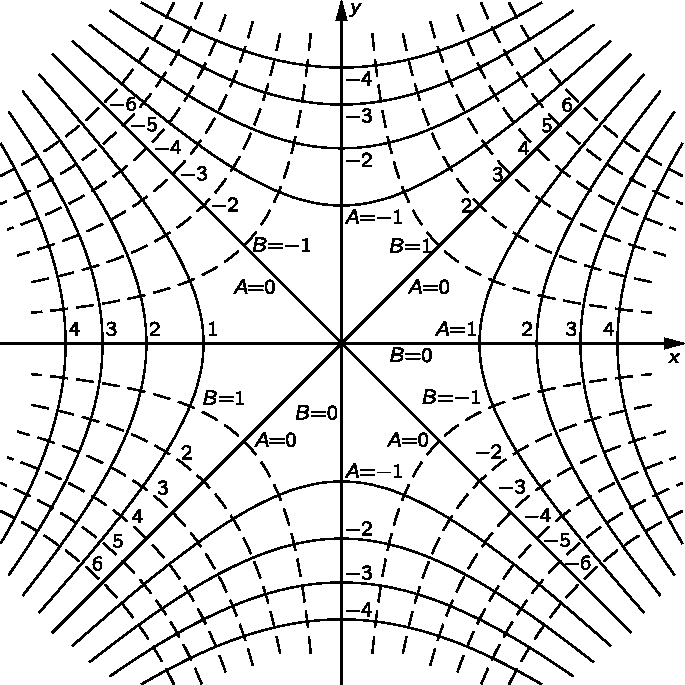
\includegraphics[width=1\linewidth]{fyz_fig170.pdf}
    \caption{Dvě soustavy ortogonálních křivek, které mohou představovat ekvipotenciální hladiny v 
             dvojrozměrné elektrostatické úloze 
             (\cite[s.~126]{Feynman02}).}
    \label{fyz:fig170}
  \end{figure}

  Taková množina ekvipotenciálních ploch odpovídá několika možným fyzikálním situacím. Zaprvé,
  představuje jemné detaily pole blízko středu mezi dvěma stejnými náboji. Zadruhé, představuje pole
  v rohu vytvořeném dvěma na sebe kolmými vodivými rovinami. Máme-li dvě elektrody takového tvaru
  jako na obr. \ref{fyz:fig171}, jež mají nestejné potenciály, bude pole v blízkosti rohu označeného
  \(C\) vypadat právě tak jako pole nad počátkem souřadnicové soustavy na obr. \ref{fyz:fig170}.

  \begin{figure}[ht!]  %\ref{fyz:fig171}
    \centering
    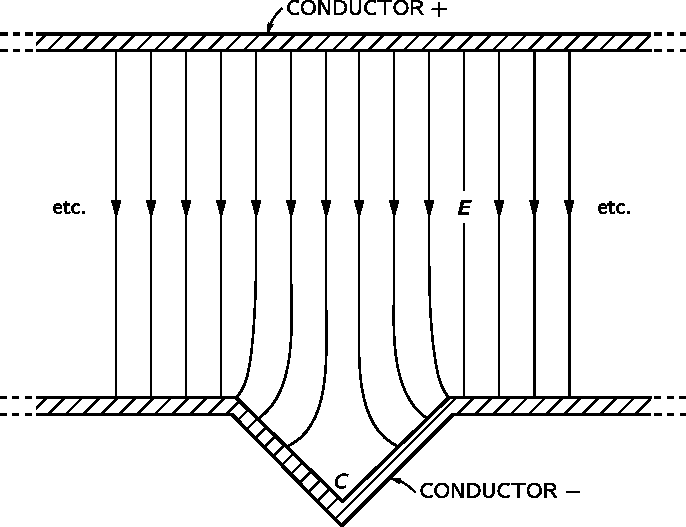
\includegraphics[width=0.9\linewidth]{fyz_fig171.pdf}
    \caption{Pole v blízkosti bodu \(C\) je stejn0 jako pole na obr. \ref{fyz:fig170}
             (\cite[s.~127]{Feynman02}).}
    \label{fyz:fig171}
  \end{figure}

  Souvislé čáry znázorňují ekvipotenciální plochy a na ně kolmé čárkované křivky jsou siločáry pole
  \(E\). Zatímco u hrotů nebo výčnělků elektrické pole roste, v prohlubních nebo jámách
  \emph{slábne}.

  Řešení, které jsme našli, odpovídá také poli elektrody hyperbolického tvaru blízko pravoúhlého
  rohu nebo poli dvou hyperbol s vhodnými potenciály. Všimněme si, že pole na obr. \ref{fyz:fig170}.
  má zajímavou vlastnost. Jeho \(x\)-ovou složku \(E_x\) vyjadřuje vztah
  \begin{equation*}
    E_x = - \diffp{\varphi}{x} = -2x
  \end{equation*}

  \begin{figure}[ht!]  %\ref{fyz:fig172}
    \centering
    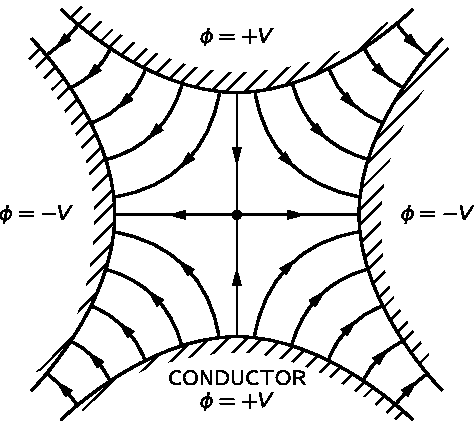
\includegraphics[width=0.9\linewidth]{fyz_fig172.pdf}
    \caption{Pole kvadrupólové čočky (\cite[s.~127]{Feynman02}).}
    \label{fyz:fig172}
  \end{figure}

  Elektrické pole je přímo úměrné vzdálenosti od osy. Tato skutečnost je využívána na výrobu
  zařízení (nazvaných kvadrupólové čočky), které se uplatňují při soustřeďování svazků částic do
  ohniska (viz článek \ref{fyz:IIchapXXIXsecVII}). Potřebné poleje obvykle vytvořeno pomocí čtyř
  elektrod hyperbolického tvaru tak, jak ukazuje obr. \ref{fyz:fig172}. Co se týče siločar
  elektrického pole ukázaných na obr. \ref{fyz:fig172}, prostě jsme z obr. \ref{fyz:fig170}
  okopírovali množinu čárkovaných křivek, jimž přísluší \(V=\text{konst}\). Dostali jsme je docela
  zadarmo.

  Z rovnic (\ref{fyz:eq835a}) a (\ref{fyz:eq835b}) vyplývá, že křivky pro \(V=\text{konst}\) jsou
  kolmé na křivky pro \(U= \text{konst}\).
  
  Jakmile zvolíme funkci \(F(\mathfrak{z})\), z \(U\) a \(V\) dostaneme jak ekvipotenciální plochy,
  tak i siločáry. Teď už budeme vědět, že jsme řešili jednu ze dvou úloh, podle toho, jakou množinu
  křivek vezmeme jako ekvipotenciální plochy.

  Jako druhý příklad uvažujme funkci
  \begin{equation}\label{fyz:eq836}
    F(\mathfrak{z}) = \sqrt{\mathfrak{z}}.
  \end{equation}
  Píšeme-li \(\mathfrak{z} = x + \imath y = \varrho e^{\imath\vartheta}\) kde \(\varrho = \sqrt{x^2
  + y^2}\) a \(\tan\vartheta = y/x\), máme
  \begin{equation*}
    F(\mathfrak{z}) = ρ^{\frac{1}{2}}e^{\imath\frac{θ}{2}} 
                    = ρ^\frac{1}{2}\left(\cos\dfrac{θ}{2}+\imath\sin\dfrac{θ}{2}\right),
  \end{equation*}
  odkud
  \begin{equation}\label{fyz:eq837}
    F(\mathfrak{z})=\left[\dfrac{(x^2 + y^2)^\frac{1}{2} + x}{2}\right]^\frac{1}{2} 
            + \imath\left[\dfrac{(x^2 + y^2)^\frac{1}{2} − x}{2}\right]^\frac{1}{2}.
  \end{equation}

  \begin{figure}[ht!]  %\ref{fyz:fig173}
    \centering
    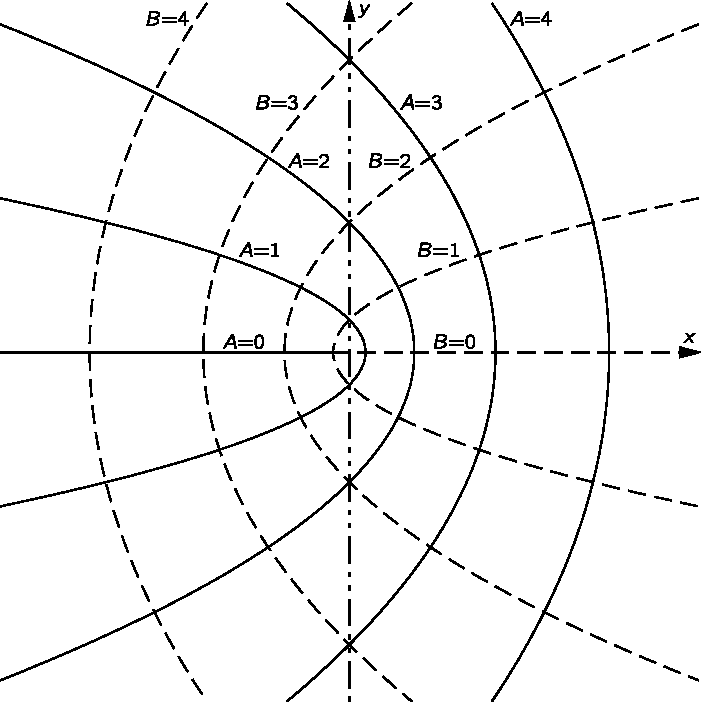
\includegraphics[width=0.9\linewidth]{fyz_fig173.pdf}
    \caption{Křivky konstantních hodnot \(U(x, y)\) a \(V(x, y)\) ze vztahu **
             (\cite[s.~128]{Feynman02}).}
    \label{fyz:fig173}
  \end{figure}

  Na obr. \ref{fyz:fig173} jsou nakresleny křivky pro \(U(x,y)=A\) a \(V(x,y) = B\), přičemž \(U\)
  a \(V\) jsou určeny pravou stranou vztahu (\ref{fyz:eq837}). Opět existuje mnoho možných situací,
  které lze těmito poli popsat. Jednou z nejzajímavějších je pole v blízkosti okraje tenké desky.
  Představuje-li přímka \(B = 0\), vpravo od osy \(y\), tenkou nabitou desku, siločáry v její
  blízkosti jsou dány křivkami pro různé hodnoty \(A\). Tuto fyzikální situaci ukazuje obr.
  \ref{fyz:fig174}.

  \begin{figure}[ht!]  %\ref{fyz:fig174}
    \centering
    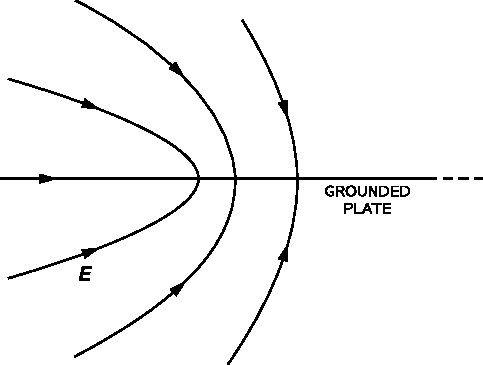
\includegraphics[width=0.8\linewidth]{fyz_fig174.pdf}
    \caption{Elektrické pole při okraji tenké uzemněné desky
             (\cite[s.~128]{Feynman02}).}
    \label{fyz:fig174}
  \end{figure}

  Další příklady jsou
  \begin{equation}\label{fyz:eq838}
    F(\mathfrak{z}) = \mathfrak{z}^\frac{3}{2},
  \end{equation}
  která dává pole na \emph{vnější} straně pravoúhlého rohu,
  \begin{equation}\label{fyz:eq839}
    F(\mathfrak{z}) = \log\mathfrak{z},
  \end{equation}
  jež dává pole nabité přímky a
  \begin{equation}\label{fyz:eq840}
    F(\mathfrak{z}) = \dfrac{1}{\mathfrak{z}},
  \end{equation}
  které odpovídá poli dvojrozměrného analogu elektrického dipólu, tj. dvou rovnoběžných opačně
  nabitých přímek nacházejících se velmi blízko u sebe. Musíme pouze zdůraznit, že ačkoliv je metoda
  komplexní proměnné velmi často účinná, je omezena pouze na dvojrozměrné úlohy; kromě toho jde o
  metodu nepřímou.
  
\section{Kmity v plazmatu}\label{fyz:IIchapVsecXXIV} 
  Nyní se budeme zabývat některými fyzikálními situacemi, v nichž pole není určeno ani pevnými
  náboji, ani náboji na vodivých plochách, ale kombinací obou faktorů. Jinými slovy, pole se bude
  chovat současně podle dvou soustav rovnic:
  \begin{enumerate}
    \item Rovnice elektrostatiky, jež uvádějí do vztahu elektrická pole s rozdělením nábojů.
    \item Rovnice z jiné části fyziky, určující polohy nebo pohyby nábojů v poli.
  \end{enumerate}

  První příklad, o kterém budeme hovořit, je dynamický. Pohyb nábojů je v něm řízen Newtonovými
  zákony. Jednoduchý příklad takové situace se vyskytuje v plazmatu, ionizovaném plynu skládajícím
  se z iontů a volných elektronů rozložených v nějaké oblasti v prostoru. Příkladem takového
  plazmatu je vrchní vrstva atmosféry, ionosféra. Ultrafialové záření ze Slunce vyráží z molekul
  vzduchu elektrony a vytváří volné elektrony a ionty. V takovém plazmatu jsou kladné ionty mnohem
  těžší než elektrony, takže v porovnání s pohybem elektronů můžeme pohyb iontů zanedbat
  
  \begin{figure}[ht!]  %\ref{fyz:fig175}
    \centering
    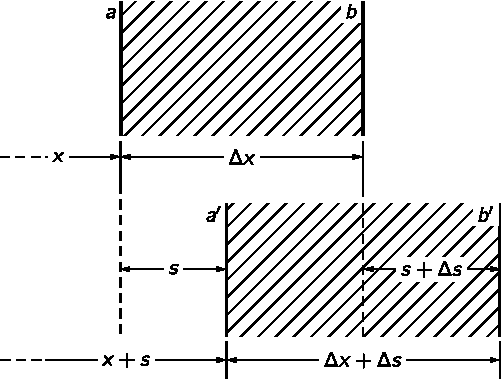
\includegraphics[width=0.9\linewidth]{fyz_fig175.pdf}
    \caption{Pohyb při vlnění v plazmatu. Elektrony v rovině \(a\) se posunou do \(a'\) a 
             elektrony v \(b\) do \(b'\)
             (\cite[s.~130]{Feynman02}).}
    \label{fyz:fig175}
  \end{figure}

  Nechť \(n_0\) je hustota elektronů v neporušeném, rovnovážném stavu. Stejná musí být i hustota
  kladných iontů, neboť plazma je elektricky neutrální (v neporušeném stavu). Nyní předpokládejme,
  že elektrony se ze svých rovnovážných poloh nějak pohnuly, a zkoumejme, co se stane. Vzroste-li v
  některé oblasti hustota elektronů, budou se vzájemně odpuzovat se snahou vrátit se do svých
  rovnovážných poloh. Při pohybu do původních poloh jejich kinetická energie vzrůstá a místo aby se
  ve své rovnovážné konfiguraci zastavily, budou se pohybovat dál. Budou okolo ní kmitat na jednu i
  na druhou stranu. Situace je podobná jako u zvukových vln, kde zpětnou silou je tlak plynu. V
  případě plazmatu je zpětnou silou elektrická síla působící na elektrony.

  Abychom naše úvahy zjednodušili, budeme se zajímat pouze o případ, kdy jsou všechny pohyby
  orientovány v jednom směru, dejme tomu ve směru osy \(x\). Předpokládejme, že elektrony,
  nacházející se původně v bodě \(x\) jsou v čase \(t\) posunuté ze svých rovnovážných poloh o malou
  vzdálenost \(s(x, t)\). Protože elektrony se posunuly, jejich hustota se obecně změnila. Změnu
  hustoty lze snadno vypočítat. Všimneme-li si obr. \ref{fyz:fig175}, vidíme, že elektrony,
  nacházející se původně mezi dvěma rovinami \(a\), \(b\), se posunuly a nyní jsou v prostoru mezi
  rovinami \(a'\), \(b'\). Počet elektronů, které se nacházely mezi \(a\), \(b\) je přímo úměrný
  hodnotě \(n_0\Delta x\) tentýž počet nyní zabírá úsek, jehož šířka je \(\Delta x + \Delta s\).
  Hustota se tedy změnila na hodnotu
  \begin{equation}\label{fyz:eq841}
    n=\dfrac{n_0Δx}{Δx+Δs}=\dfrac{n_0}{1+(Δs/Δx)}.
  \end{equation}
  Je-li změna hustoty malá, můžeme psát (rozvineme-li \((1 + \varepsilon)^{-1}\) do binomické řady)
  \begin{equation}\label{fyz:eq842}
    n=n_0\left(1−\dfrac{Δs}{Δx}\right)
  \end{equation}
  Předpokládáme, že kladné ionty se významněji nepohnou (v důsledku jejich mnohem větší
  setrvačnosti), takže jejich hustota zůstává \(n_0\). Každý elektron nese náboj - \(q_e\) takže
  střední hustotu náboje v kterémkoli bodě vyjadřuje vztah
  \begin{align}
    ρ&=−(n−n_0)q_e,        \nonumber\\
    \shortintertext{resp.}
    ρ&=n_0q_e\diff{s}{x}   \label{fyz:eq843}
  \end{align}
  (kde \(\Delta S/\Delta t\) jsme napsali v diferenciálním tvaru).

  Hustota náboje souvisí s elektrickým polem podle Maxwellových rovnic. Tedy
  \begin{equation}\label{fyz:eq844}
    \nabla\cdot\vec{E} = \dfrac{ρ}{\varepsilon_0}
  \end{equation}
  Jde-li opravdu o jednorozměrný problém (a nejsou-li žádná jiná pole kromě toho, jež bylo vyvoláno
  posunem elektronů), elektrické pole \(\vec{E}\) má jedinou složku \(E_x\). Po dosazení
  (\ref{fyz:eq843}) do rovnice (\ref{fyz:eq844}) pak dostaneme
  \begin{align}
    \diffp{E_x}{x} &= \dfrac{n_0q_e}{\varepsilon_0}\diffp{s}{x}.   \label{fyz:eq845}  \\
    \shortintertext{Integrováním \ref{fyz:eq845} najdeme}
    E_x            &=\dfrac{n_0q_e}{\varepsilon_0}s+K.             \label{fyz:eq846} 
  \end{align}
  Je-li \(S = 0\), pak \(E_x =0\) a integrační konstanta \(K\) je tedy rovna nule. 
  
  V posunuté poloze působí na elektron síla
  \begin{equation}\label{fyz:eq847} 
    F_x=−\dfrac{n_0q^2_e}{\varepsilon_0}s.
  \end{equation}
  Jde tedy o zpětnou sílu přímo úměrnou posunutí s elektronu. To vede k harmonickým kmitům
  elektronů. Pohybová rovnice posunutého elektronu je
  \begin{equation}\label{fyz:eq848} 
    m_e\diff[2]{s}{t} = −\dfrac{n_0q^2_e}{\varepsilon_0}s.
  \end{equation}
  Vidíme, že \(s\) se bude měnit harmonicky. Závislost \(s\) na čase bude udávat funkce \(\cos\omega
  t\) nebo použijeme-li exponenciální symboliku z \ref{part:FYZI}. dílu, funkce
  \begin{equation*}
  e^{\imath ω_pt}.
  \end{equation*}
  Úhlovou frekvenci kmitů \(ω_p\) určuje rovnice (\ref{fyz:eq848}), podle níž
  \begin{equation}\label{fyz:eq849} 
  ω^2_p=\dfrac{n_0q^2_e}{\varepsilon_0m_e},
  \end{equation}
  Veličina \(ω_p\) se nazývá \textbf{elektronová plazmová úhlováf rekvence}. Jde o charakteristickou
  hodnotu pro plazma.

  Příslušné veličiny jsou často vyjadřovány pomocí veličiny \(e^2\) definované takto:
  \begin{equation}\label{fyz:eq850} 
    e^2=\dfrac{q^2_e}{4π\varepsilon_0}=\SI{2.3068e-28}{\newton\square\m}.
  \end{equation}
  V této konvenci bude mít vztah (\ref{fyz:eq849}) tvar
  \begin{equation}\label{fyz:eq851} 
    ω^2_p=\dfrac{4πe^2n_0}{m_e},
  \end{equation}

  Tak jsme zjistili, že porucha plazmatu vyvolá volné kmity elektronů kolem jejich rovnovážných
  poloh s vlastní úhlovou frekvencí \(ω_p\), která je přímo úměrná odmocnině hustoty elektronů.
  Elektrony se v plazmatu chovají jako rezonanční soustava podobná soustavám popsaným v
  \ref{fyz:IchapXXIII}. kapitole \ref{part:FYZI}. dílu.

  Vlastní rezonance plazmatu vede k některým zajímavým efektům. Například při šíření rádiových vln
  ionosférou se zjišťuje, že mohou procházet pouze tehdy, je-li jejich frekvence vyšší než frekvence
  plazmová. V opačném případě se signál odrazí zpět. Chceme-li komunikovat s družicí ve vesmíru,
  musíme použít vysoké frekvence. Ale když chceme komunikovat s radiostanicí za obzorem, musíme
  použít nižší frekvence kmitů v plazmatu, aby se signál odrazil zpět k zemi. 
  
  Jiný zajímavý příklad kmitů v plazmatu se vyskytuje v kovech. Kov obsahuje plazma kladných iontů a
  volných elektronů. Hustota \(n_0\) je tam velmi velká, a velká je tedy i úhlová frekvence\(ω_p\).
  Naproti tomu lze kmity elektronů ještě pozorovat. Podle kvantové mechaniky má harmonický oscilátor
  s vlastní úhlovou frekvencí \(ω_p\) hladiny energie vzdálené od sebe o přírůstek \(ℏω_p\).
  Ostřeluje-li se tedy elektrony řekněme hliníková fólie a velmi pečlivě se měří energie elektronů
  za ní, lze čekat, že v důsledku kmitů v plazmatu ztratí některé z elektronů energii \(ℏω_p\). To
  se skutečně stává. Roku 1936 se poprvé experimentálně pozorovalo, že elektrony s energiemi od
  několika set do několika tisíců elektronvoltů ztrácejí při rozptylu na tenké kovové fólii nebo při
  průchodu skrz ní energii skokem. Tento jev byl objasněn až r. 1953, když Bohm a Pines ukázali,
  že pozorování je možné vysvětlit kvantovým buzením kmitů v plazmatu kovu.

\section{Koloidní částice v elektrolytu}\label{fyz:IIchapVsecXXV}
  Přikročíme k dalšímu jevu, v němž polohy nábojů určuje potenciál, vytvořený částečně týmiž náboji.
  Efekty, které z toho vyplývají, důležitým způsobem ovlivňují chování koloidů. Koloid představuje
  vodní suspenzi malých nabitých částic, jež, ačkoliv jsou mikroskopické, jsou ve srovnání s atomy
  velmi velké. Kdyby koloidní částice nebyly nabité, jevily by tendenci srážet se do velkých celků;
  působením svých nábojů se navzájem odpuzují a zůstávají ve formě suspenze.

  Je-li kromě toho ve vodě rozpuštěna ještě nějaká sůl, bude disociována na kladné a záporné ionty.
  (Takový roztok se nazývá elektrolyt.) Záporné ionty se přitahují ke koloidním částicím (o nichž
  předpokládáme, že mají kladný náboj) a kladné ionty jsou jim i odpuzovány. Budeme zkoumat, jak
  jsou ionty obklopující takovou koloidní částici rozděleny v prostoru.

  Pro jednoduchost budeme opět řešit pouze jednorozměrný případ. Představíme-li si koloidní částici
  jako kouli s velmi velkým poloměrem (v rozměrech atomů!), můžeme malou část jejího povrchu
  považovat za rovinu. (Vždy, když se někdo snaží pochopit nový jev, je dobré zkoumat snad až trochu
  přehnaně zjednodušený model jevu; po pochopení problému s tímto modelem je člověk lépe připraven
  pustit se do exaktnějšího výpočtu.)

  Předpokládáme, že rozdělení iontů generuje hustotu náboje \(ρ(x)\) a elektrický potenciál \(ϕ\),
  souvisící podle elektrostatického zákona \(∇^2ϕ=−ρ/\varepsilon_0\), anebo v případě polí, která se mění
  pouze v jednom rozměru, podle vztahu
  \begin{equation}\label{fyz:eq852}
    \diff[2]{ϕ}{x} = −\dfrac{ρ}{\varepsilon_0}.
  \end{equation}

  Nyní předpokládejme takový potenciál a ptejme se, jak by se v něm ionty rozdělily. Určit to můžeme
  na základě principů statistické mechaniky. Náš problém spočívá v určení \(ϕ(x)\) tak, aby výsledná
  hustota náboje ze statistické mechaniky vyhovovala i vztahu (\ref{fyz:eq852}).

  Podle statistické mechaniky (viz kapitola \ref{fyz:IchapXL}, díl \ref{part:FYZI} jsou částice
  nacházející se v tepelné rovnováze v silovém poli rozděleny tak, že jejich hustotu \(n\) v poloze
  \(x\) vyjadřuje vztah
  \begin{equation}
    n(x)=n_0e^{−U(x)/kT},
  \end{equation}
  kde \(U(x)\) je potenciální energie, \(k\) Boltzmannova konstanta a \(T\) absolutní teplota.
  
  Předpokládáme, že ionty nesou po jednom elektronovém náboji \(q_e\), ať už kladném nebo záporném.
  Ve vzdálenosti \(x\) od povrchu koloidní částice bude mít kladný ion potenciální energii
  \(q_eϕ(x)\), takže
  \begin{equation*}
    U(x)=q_eϕ(x).
  \end{equation*}
  Hustota kladných iontů \(n_+\) je potom
  \begin{equation*}
    n_+(x)=n_0e^{−q_eϕ(x)/kT}.
  \end{equation*}
  Podobně je vyjádřena hustota záporných iontů
  \begin{equation*}
    n_−(x)=n_0e^{+q_eϕ(x)/kT}.
  \end{equation*}
  Celková hustota náboje je
  \begin{equation*}
    ρ=q_en_+ −qen−,
  \end{equation*}
  resp.
  \begin{equation}\label{fyz:eq853}
    ρ=q_en_0\left(e^{−q_eϕ/kT}−e^{+q_eϕ/kT}\right).
  \end{equation}
  Dosazením tohoto výrazu do (\ref{fyz:eq852}) dostaneme, že potenciál \(ϕ\) musí splňovat rovnici
  \begin{equation}\label{fyz:eq854}
    \diff[2]{ϕ}{x} =−\dfrac{q_en_0}{\varepsilon_0}\left(e^{−q_eϕ/kT}−e^{+q_eϕ/kT}\right).
  \end{equation}
  Tuto rovnici je možné snadno řešit obecně (obě strany vynásobte výrazem \(2(\diff{ϕ}{x})\) a pak
  integrujte podle \(x\)), ale abychom úlohu co nejvíc zjednodušili, budeme uvažovat pouze limitní
  případ, v němž jsou potenciály malé, nebo teplota \(T\) je vysoká. Případ malého \(ϕ\) odpovídá
  zředěnému roztoku. V těchto případech je exponent malý a můžeme provést aproximaci
  \begin{equation}\label{fyz:eq855}
    e^{±q_eϕ/kT}=1±\dfrac{q_e}{kT}ϕ.
  \end{equation}
  Rovnice (\ref{fyz:eq854}) má potom tvar
  \begin{equation}\label{fyz:eq856}
    \diff[2]{ϕ}{x}=+\dfrac{2n_0q^2_e}{\varepsilon_0kT}ϕ(x).
  \end{equation}
  Všimněme si, že pravá strana má tentokrát kladné znaménko. Rovnice tedy nemá oscilující, ale 
  exponenciální řešení pro \(ϕ\).
  
  Obecné řešení rovnice (\ref{fyz:eq856}) má tvar
  \begin{equation}\label{fyz:eq857}
    ϕ=Ae^{−x/D}+Be^{+x/D},
  \end{equation}
  kde
  \begin{equation}\label{fyz:eq858}
    D^2=\dfrac{\varepsilon_0kT}{2n_0q^2_e}.
  \end{equation}
  Konstanty \(A\) a \(B\) je třeba určit z podmínek úlohy. V našem případě \(B\) musí být rovno
  nule; jinak by pro velké \(x\) potenciál rostl do nekonečna. Bude tedy
  \begin{equation}\label{fyz:eq859}
    ϕ=Ae^{−x/D},
  \end{equation}
  kde \(A\) je potenciál v poloze \(x = 0\), tj. na povrchu koloidní částice.

  \begin{figure}[ht!]  %\ref{fyz:fig176}
    \centering
    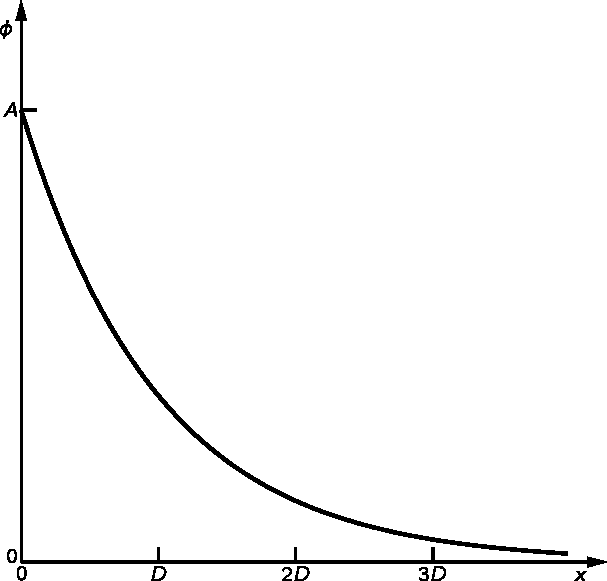
\includegraphics[width=0.7\linewidth]{fyz_fig176.pdf}
    \caption{Průběh potenciálu u povrchu koloidní částice. \(D\) je Debyeova délka
             (\cite[s.~134]{Feynman02}).}
    \label{fyz:fig176}
  \end{figure}

  Při zvětšení vzdálenosti o \(D\) se potenciál zmenší v poměru \(1/e\), jak je vidět z grafu na
  obr. \ref{fyz:fig176}. Veličina \(D\) se nazývá \textbf{Debyeova délka}. Je mírou tloušťky
  iontového obalu, jenž obklopuje velkou nabitou částici v elektrolytu. Podle vztahu
  (\ref{fyz:eq859}) se obal ztenčuje, když koncentrace iontů \(n_0\) vzrůstá nebo teplota klesá.

  Konstantu \(A\) ve vztahu (\ref{fyz:eq859}) snadno určíme, známe-li \(σ\) plošný náboj na povrchu
  koloidní částice. Víme, že
  \begin{equation}\label{fyz:eq860}
    E_n=E_x(0)=\dfrac{σ}{\varepsilon_0}.
  \end{equation}
  Ale \(\vec{E}\) je i gradientem \(ϕ\).
  \begin{equation}\label{fyz:eq861}
    E_x(0)=−\left.\diffp{ϕ}{x}\right\rvert_0=+\dfrac{A}{D},
  \end{equation}
  z čehož dostáváme, že
  \begin{equation}\label{fyz:eq862}
    A=\dfrac{σD}{\varepsilon_0}.
  \end{equation}
  Dosadíme-li tento výsledek do (\ref{fyz:eq859}), najdeme (při \(x=0\)) výraz pro potenciál
  koloidní částice:
  \begin{equation}\label{fyz:eq863}
    ϕ(0)=\dfrac{σD}{\varepsilon_0}.
  \end{equation}
  Všimněme si, že je to stejný vztah jako pro rozdíl potenciálu na deskách rovinného kondenzátoru se
  vzájemnou vzdáleností desek \(D\) a plošnou hustotou náboje \(σ\).
 
  Řekli jsme, že koloidní částice jsou jedna od druhé separovány v důsledku jejich elektrického
  odpuzování. Nyní však vidíme, že už v malé vzdálenosti od povrchu částice je pole zeslabeno
  iontovým obalem, jenž ji obklopuje. Stanou-li se obaly dostatečné tenkými, budou mít částice
  dobrou šanci se srazit - potom splynou a koloid se z kapaliny vysráží. Z naší analýzy je jasné,
  proč by přidání dostatečného množství soli do koloidu způsobilo jeho vysrážení. Tento proces se
  nazývá vysolování koloidu.

  Jiným zajímavým příkladem je účinek, který má roztok soli na proteinové molekuly. Molekula
  proteinu představuje dlouhý, složitý a ohybný řetězec aminokyselin. Nese různé náboje a někdy se
  stává, že existuje výsledný, řekněme záporný náboj, který je rozdělen podél řetězce. V důsledku
  vzájemného odpuzování záporných nábojů zůstane proteinový řetězec napnutý. Kromě toho, nachází-li
  se v roztoku jiné podobné řetězové molekuly, budou týmiž odpudivými účinky udržovány navzájem
  odděleny. To umožňuje existenci suspenze řetězových molekul v kapalině. Ale přidáme-li do kapaliny
  sůl, vlastnosti suspenze změníme. Po přidání soli do roztoku a tím vyvolaném zmenšení Debyeovy
  délky řetězové molekuly se mohou jedna ke druhé přiblížit a mohou se také svinout. Přidá-li se do
  roztoku dostatek soli, řetězové molekuly se z roztoku vysrážejí. Existuje mnoho chemických jevů
  tohoto druhu, které lze pochopit na základě elektrických sil.

\section{Elektrostatické pole mřížky}\label{fyz:IIchapVsecXXVI} 
  Jako náš poslední příklad bychom rádi vysvětlili ještě jednu zajímavou vlastnost elektrických
  polí. Je to vlastnost, jež se využívá při návrhu elektrických přístrojů, při konstrukci elektronek
  a pro jiné účely. Jde o charakter elektrického pole blízko mřížky z nabitých drátů. Abychom úlohu
  co nejvíc zjednodušili, uvažujme o řadě rovnoběžných drátů ležících v rovině. Dráty, nechť jsou
  nekonečně dlouhé a jeden od druhého stejně vzdálené.

  Prozkoumáme-li pole ve velké vzdálenosti nad rovinou drátů, zjistíme, že jde o konstantní
  elektrické pole právě takové, jako kdyby náboj byl v rovině rozdělen rovnoměrně. Při přibližování
  k mřížce se charakter pole začíná odchylovat od homogennosti, kterou jsme zjistili ve velké
  vzdálenosti od mřížky. Chtěli bychom vypočítat, v jaké vzdálenosti od mřížky se objeví větší
  výkyvy potenciálu. Obrázek \ref{fyz:fig177} představuje hrubý náčrt ekvipotenciálních ploch v
  různých vzdálenostech od mřížky. Čím blíž jsme k mřížce, tím jsou výkyvy větší. Pohybujeme-li se
  rovnoběžně s mřížkou, pozorujeme, že pole kolísá periodicky.

  \begin{figure}[ht!]  %\ref{fyz:fig177}
    \centering
    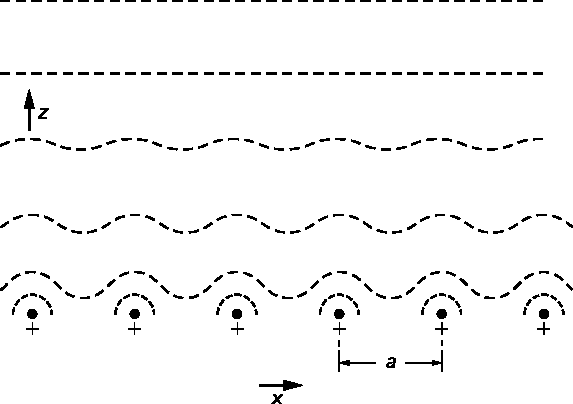
\includegraphics[width=0.7\linewidth]{fyz_fig177.pdf}
    \caption{Ekvipotenciální plochy nad pravidelnou mřížkou nabitých drátů
             (\cite[s.~136]{Feynman02}).}
    \label{fyz:fig177}
  \end{figure}

  Viděli jsme (kapitola \ref{fyz:IchapL}, díl \ref{part:FYZI}), že každou periodickou veličinu je
  možné vyjádřit jako součet sinusových vln (Fourierova věta). Podívejme se, zdaje možno najít
  vhodnou harmonickou funkci, která splňuje rovnice pole.

  Jsou-li dráty umístěny v rovině \(xy\) rovnoběžně s osou \(y\), mohli bychom zkusit členy tvaru
  \begin{equation}\label{fyz:eq864}
    ϕ(x,z)=F_n(z)\cos\dfrac{2πnx}{a},
  \end{equation}
  kde \(a\) je mezera mezi dráty a \(n\) je řád harmonické. (Předpokládali jsme dlouhé dráty, takže
  by se neměla projevit žádná závislost na \(y\).) Úplné řešení lze napsat jako suma takových členů
  pro \(n= 1,2,3,\ldots\)

  Má-li jít o platný potenciál, musí v oblasti nad dráty (kde nejsou žádné náboje) splňovat
  Laplaceovu rovnici, tj. musí být
  \begin{equation}\label{fyz:eq891}
    \diffp[2]{ϕ}{x} + \diffp[2]{ϕ}{z} = 0. 
  \end{equation}
  Když do této rovnice dosadíme výraz (\ref{fyz:eq864}), zjistíme, že
  \begin{equation}\label{fyz:eq865}
    −\dfrac{4π^2n^2}{a^2}F_n(z)\cos\dfrac{2πnx}{a}+\diff[2]{F_n}{z}\cos\dfrac{2πnx}{a}=0, 
  \end{equation}
  tj. \(F_n(x)\) že musí vyhovovat rovnici
  \begin{equation}\label{fyz:eq866}
    \diff[2]{F_n}{z}= \dfrac{4π^2n^2}{a^2}F_n.
  \end{equation}
  Musí tedy platit
  \begin{equation}\label{fyz:eq800} 
    F_n=A_ne^{−z/z_0},
  \end{equation}
  kde
  \begin{equation}\label{fyz:eq867}
    z_0=\dfrac{a}{2πn}.
  \end{equation}  
  Zjistili jsme tedy, že existuje-li Fourierova složka pole s \(n\)-tou harmonickou, bude se s
  výškou nad mřížkou exponenciálně zmenšovat s charakteristickou vzdáleností \(z_0=a/2πn\).
  Amplituda první harmonické (\(n=l\)) se zmenší \(e^{−2π}\)-krát při vzrůstu \(z\) o jednu
  mřížkovou konstantu \(a\) (prudký pokles). Další harmonické klesají při vzdalování od mřížky ještě
  rychleji. Vidíme, že jsme-li jen několik vzdáleností \(a\) od mřížky, je pole téměř homogenní, tj.
  oscilující členy jsou malé. Vždy tam, samozřejmě, zůstane pole nulové harmonické
  \begin{equation*}
    ϕ_0=−E_0z
  \end{equation*}
  které přechází v homogenní pole při velkém \(z\). Úplné řešení dostaneme vypočítáním tohoto členu
  se sumou členů tvaru (\ref{fyz:eq864}), přičemž \(F_n\) se vezme ze vztahu (\ref{fyz:eq800} ).
  Koeficienty \(A_n\) jsou zvoleny tak, aby výsledná suma po zderivování dala elektrické pole, které
  odpovídá hustotě náboje rna drátech tvořících mřížku.
  
  Touto námi právě vypracovanou metodou lze vysvětlit, proč elektrostatické stínění pomocí sítě je
  často stejně dobré jako stínění pomocí souvislého kovového plechu. Pole uvnitř uzavřené sítě bude
  nulové s výjimkou takových míst, jejichž vzdálenosti od sítě nepřevyšují několik mezer mezi jejími
  dráty. Nyní vidíme, proč se na ochranu citlivého elektrického zařízení před vnějšími rušivými poli
  často používá měděná síť - je lehčí a levnější než měděný plech.